\documentclass[11pt, a4paper, oneside]{report}
\pdfoutput=1
\usepackage{preamble}
 % !TEX root = main.tex
%=======================================================================
\begin{document}

\begin{titlepage}
\AddToShipoutPicture*{\put(0,0){\includegraphics*{nat-farve}}}
\AddToShipoutPicture*{\put(0,0){\includegraphics*{nat-en}}}

\begin{flushleft}
\vspace*{3cm}
\textbf{\huge{Master's Thesis}}

\vspace*{3mm}
\textbf{Martin Holm Cservenka} \\
Department of Computer Science \\
University of Copenhagen \\
\texttt{djp595@alumni.ku.dk} 


\vspace*{4cm}
\textbf{\huge{Design and Implementation of Dynamic Memory Management in a Reversible Object-Oriented Programming Language}}
\vfill
\textbf{Supervisors:} Robert Glück \& Torben Ægidius Mogensen

\textbf{Submitted:} January $25^{th}$, 2018

Revision 1.01
\end{flushleft}
\end{titlepage}

\newpage 

\begin{versionhistory}
  \vhEntry{0.1}{2017-05-02}{Martin}{\rooplpp design and heap design discussion}
  \vhEntry{0.2}{2017-05-16}{Martin}{Updated front-page logo and expanded heap design section}
  \vhEntry{0.3}{2017-05-24}{Martin}{Added Fragmentation and Garbage subsection. Added assumption about available heap manipulation subroutines for heap layout section. Added explanations of listings. Expanded Buddy-memory \texttt{get\_free} algorithm with early idea for heap splitting/merging and heap growth}
  \vhEntry{0.4}{2017-06-24}{Martin}{Extended grammar in section~\ref{sec:syntax}. Added sections~\ref{sec:object-instantiation} to~\ref{sec:local-blocks}. Addressed Chapter~\ref{chp:compilation} feedback. Rewrote pseudo-code algorithms in \textsc{Extended Janus}.}
  \vhEntry{0.5}{2017-10-11}{Martin}{Finalized a few sections in chapter~\ref{chp:introduction}. Update chapter~\ref{chp:compilation} to reflect work done on compiler.}
  \vhEntry{0.6}{2017-10-12}{Martin}{Added first version of section~\ref{sec:object-allocation-deallocation}}
  \vhEntry{0.7}{2017-10-25}{Martin}{Moved Dynamic Memory Management sections into their own chapter~\ref{chp:dynamic-memory-management}. Added computation strength section~\ref{sec:computational-strength}}
  \vhEntry{0.8}{2017-11-07}{Martin}{Added section~\ref{sec:type-system} and~\ref{sec:language-semantics}. Started on section~\ref{sec:program-inversion}. Updated RTM in section~\ref{sec:computational-strength}.}
  \vhEntry{0.9}{2017-12-15}{Martin}{Wrote section~\ref{sec:local-blocks}, finished remaining sections of chapter~\ref{chp:introduction}, addressed feedback in chapter~\ref{chp:rooplpp} (sections~\ref{sec:type-system},~\ref{sec:language-semantics}), updated syntax for updated arrays in section~\ref{sec:syntax}, revised array sections to current implementation in section~\ref{sec:array-model} and~\ref{sec:array-instantiation}. Updated type system and semantics with array specific rules in section~\ref{sec:type-system} and~\ref{sec:language-semantics}. Started on section~\ref{sec:error-handling}.}
  \vhEntry{1.0}{2017-12-29}{Martin}{Adressed feedback in section~\ref{sec:local-blocks},~\ref{sec:rooplpp-expressiveness} and~\ref{sec:language-semantics}. Finished section~\ref{sec:program-inversion}. Updated section~\ref{sec:computational-strength} with new RTM implementation. Revised and rewrote large parts of chapter~\ref{chp:dynamic-memory-management}. Wrote section~\ref{sec:roopl-to-pisa-compiler}. Wrote section~\ref{sec:arrays} and section~\ref{sec:referencing-compilation} after finalizing compiler code. Finished section~\ref{sec:error-handling}. Wrote section~\ref{sec:implementation}. Added conclusion in chapter~\ref{chp:conclusions}. Added abstract and preface.}
  \vhEntry{1.01}{2018-01-16}{Martin}{Proofreading and minor changes. Added section~\ref{sec:evaluation}. Update RTM algorithm}
  \vhEntry{1.02}{2018-01-21}{Martin}{More Proofreading and minor changes. Updated example program in beginning of chapter~\ref{chp:rooplpp}. Reformatted reference list}
  \vhEntry{1.03}{2018-01-23}{Martin}{Added figure~\ref{fig:sugar-construct-destruct} to clarify existing description. Added figure~\ref{fig:pseudo-instructions} to describe pseudo-instructions used in chapter. Updated figure~\ref{fig:sec:program-structure} to reflect minor code changes. Added figure and description for translation of \rooplpp object blocks in section~\ref{sec:object-allocation-deallocation}. Added figure~\ref{fig:array-memory-storage} to illustrate array storage model. Added two more items that should be run-time checked in section~\ref{sec:error-handling}. Updated syntax of \textbf{construct}/\textbf{destruct} blocks to only allow objects as arrays does not make sense in section~\ref{sec:syntax}.}

\end{versionhistory}  

% TODOs:
% \begin{itemize}
  % \item Finalize Chapter~\ref{chp:introduction}
  % \item Revise section~\ref{sec:computational-strength} with updated RTM implementation and description
  % \item Finalize section~\ref{sec:program-inversion} 
  % \item Revise chapter~\ref{chp:dynamic-memory-management} and finish figures
  % \item Update chapter~\ref{chp:compilation} to reflect code updates
  % \item Describe reference counting and array implementation in chapter~\ref{chp:compilation}
  % \item Write chapter~\ref{chp:conclusions}.
  % \item Write abstract and preface
  % \item Address feedback
  % \item Proofreading :-)
  % \item Fix references


  % TODO: Validate that one allocation figure showing splits actually works IRL
% \end{itemize}

\newpage

\chapter*{Abstract}
\markright{Abstract}

The reversible object-oriented programming language (\textsc{Roopl}) was presented in late 2016 and proved that object-oriented programming paradigms works in the reversible setting. The language featured simple statically scoped objects which made non-trivial programs tedious, if not impossible to write using the limited tools provided.
We introduce an extension to \textsc{Roopl} in form the new language \rooplpp, featuring dynamic memory management and fixed-sized arrays for increased language expressiveness. The language is a superset of \textsc{Roopl} and has formally been defined by its language semantics, type system and computational universality. Considerations for reversible memory manager layouts are discussed and ultimately lead to the selection of the Buddy Memory layout. Translations of the extensions added in \rooplpp to the reversible assembly language \textsc{Pisa} are presented to provide garbage-free computations. The dynamic memory management extension successfully increases the expressiveness of \textsc{Roopl} and as a result, show that non-trivial reversible data structures, such as binary trees and doubly-linked lists, are feasible and do not contradict the reversible computing paradigm.
\newpage 

\chapter*{Preface}
\markright{Preface}

This Master's Thesis is submitted as the last part for the degree of Master of Science in Computer Science at the University of Copenhagen, Department of Computer Science, presenting a 30 ECTS workload.

The thesis consists of \pageref*{LastPage} pages and a ZIP archive containing source code and test programs developed as part of the thesis work.

I would like to thank my two supervisors, Robert Glück and Torben Mogensen, for their invaluable supervision and guidance throughout this project and introduction to the field of reversible computing. A big thanks to my university colleague and friend, Tue Haulund, for allowing me to continue his initial work on \textsc{Roopl} and providing information, sparring and source code material and for being a great ally through our years at the University of Copenhagen. In addition, thanks to my dear aunt Doris, for financially supporting my studies by paying for all my books needed. Finally, a thanks to Jess, for all the love and support throughout the entire span of my thesis process.
 
\newpage

\tableofcontents
\newpage

\listoffigures 
\newpage
 
\chapter{Introduction}
\label{chp:introduction}
In recent years, technologies such as cloud-based services, cryptocurrency mining and other services requiring large computational power and availability has been on the rise. These services are hosted on massive server parks, consuming immense amounts of electricity in order to power the machines and the cooling architectures as heat dissipates from the hardware. A recent study showed that the Bitcoin network including its mining processes' currently stands at 0.13\% of the total global electricity consumption, rivaling the usage of a small country like Denmark's~\cite{digiconomist:bitcoin}. With the recent years focus on climate and particularly energy consumption, companies have started to attempt to reduce their power usage in these massive server farms. As an example, Facebook built new server park in the arctic circle in 2013, in an attempt to take advantage of the natural surroundings in the cooling architecture to reduce its power consumption~\cite{bloomberg:facebook}. 

Reversible computing presents a possible solution the problematic power consumption issues revolving around computations. Traditional, irreversible computations dissipates heat during their computation. Landauer's principle states that deletion of information in a system always results by an increase in energy consumption. In reversible computing, all information is preserved throughout the execution, and as such, the energy consumption theoretically should be smaller~\cite{rl:irreversibility}.

Currently, reversible computing is not commercially appealing, as it is an area which still is being actively researched. However, several steps has been taken in the direction of a fully reversible system, which some day might be applicable in a large setting. Reversible machine architectures have been presented such as the Pendulum architecture and its instruction set Pendulum ISA (\textsc{Pisa})~\cite{cv:pendulum} and the \textsc{BobISA} architecture and instruction set~\cite{mt:bob} and high level languages \textsc{Janus}~\cite{cl:janus, ty:janus, ty:ejanus} and \textsc{R}~\cite{mf:r} exists. 

While cryptocurrency mining and many other computations are not reversible, the area remains interesting in terms of its applications and gains.


\section{Reversible Computing}
\label{sec:reversible-computing}
Reversible computing is a two-directional computational model in which all processes are time-invertible. This means, that at any time during execution, the computation can return to a former state. In order to maintain \textit{reversibility}, the reversible computational modal cannot compute \textit{many-to-one} functions, as the models requires an exact inverse $f^{-1}$ of a function $f$ in order to support backwards determinism. Therefore, reversible programs must only consist on \textit{one-to-one} functions, also known as \textit{injective} functions, which results in a garbage-free computations.

As each step of a reversible program is locally invertible, meaning each of its component has exactly one inverse component, a reversible program can be inverted simply by computing the inverse of each of its components, without any knowledge about the overall program's functionality or requirements. This property immediately yields interesting consequences in terms of software development, as an encryption or compression algorithm implemented in a reversible language immediately yields the decryption or decompression algorithm.

The reversibility is however not free at comes at the cost of strictness when writing programs. Almost every popular, irreversible programming language features a conditional component in form of \textbf{if}-\textbf{else}-statements. In these languages, we only define the \textit{entry}-condition in the condition, that is, the condition that determines which branch of the component we continue execution in. In reversible languages, we must also specify an \textit{exit}-condition, such that we can determine which branch we should follow, we we are executing the program in reverse. In theory, this sounds trivial, but in practice it turns to add a new layer of complexity when writing programs.


\section{Object-Oriented Programming}
\label{sec:object-oriented-programming}
Object-oriented programming (OOP) has for many years been the most widely used programming paradigm as reflected in the popular usage of object-oriented programming languages, such as the \textsc{C}-family languages, \textsc{Java}, \textsc{PHP} and in recent years \textsc{Javascript} and \textsc{Python}. Using the OOP core concepts such as \textit{inheritance}, \textit{encapsulation} and \textit{polymorphism} allows complex systems to be modeled by breaking the system into smaller parts in form of abstract objects. 


\section{Reversible Object-Oriented Programming}
\label{sec:reversible-object-oriented-programming}
The high-level reversible language \textsc{Roopl} (Reversible Object-Oriented Programming Language) was introduced in late 2016~\cite{th:roopl, th:roopl2}. The language extends the design of previously existing reversible imperative languages with object-oriented programming language features such as user-defined data types, class inheritance and subtype-polymorphism. As a first, \textsc{Roopl} successfully integrates the object-oriented programming (OOP) paradigms into the reversible computation setting using a static memory manager to maintain garbage-free computation, but at cost of "programmer usability" as objects only lives within \textbf{construct} / \textbf{deconstruct} blocks, which needs to be predefined, as the program call stacks is required to be reset before program termination.
 

\section{Motivation}
\label{sec:motivation}
\textsc{Roopl}'s block defined objects and lack of references are problematic when write complex, reversible programs using OOP methodologies. It has therefore been proposed to extend and partially redesign the language with dynamic memory management in mind, such that these shortcomings can be addressed, ultimately increasing the usability of reversible OOP. Work within the field of reversible computing related to heap manipulation~\cite{ha:heap}, reference counting~\cite{tm:refcounting} and garbage collection~\cite{tm:garbage} suggests that a \textsc{Roopl} extension is feasible.


\section{Thesis Statement}
\label{sec:thesis-statement}
An extension of the reversible object-oriented programming language with dynamic memory management is possible and effective. The resulting expressiveness allows non-trivial reversible programming previously unseen, such as reversible data structures.

\section{Outline}
\label{sec:outline}
This Master's thesis consists of four chapters, besides the introductory chapter. The following summary describes the following chapters
\begin{itemize}
    \item \textbf{Chapter 2} formally defines the \textsc{Roopl} extension in form of the new language \rooplpp, a superset of \textsc{Roopl}.
    \item \textbf{Chapter 3} serves as a brief description of dynamic memory management along with a discussion of various reversible, dynamic memory management layouts.
    \item \textbf{Chapter 4} presents the translation techniques utilized in the compiling a \rooplpp program to \textsc{Pisa} instructions.
    \item \textbf{Chapter 5} presents the conclusions of the thesis and future work proposals.
\end{itemize}

Besides the five chapters, a number of appendices is supplied, containing the source code of the \rooplpp to \textsc{Pisa} compiler, the \rooplpp source code for the example programs and their translated \textsc{Pisa} versions.
\newpage

\chapter{The \textsc{Roolp\texttt{++}} Language}
\label{chp:rooplpp}
With the design and implementation of the \textsc{Reversible Object-Oriented Programming Language} (\textsc{Roopl}), the first steps into the uncharted lands of Object-Oriented Programming (OOP) and reversibility was taken. In this chapter, we will present \rooplpp, the natural successor of \textsc{Roopl}, improving the language's object instantiation by letting objects live outside \texttt{construct / deconstruct} blocks, allowing complex, reversible programs to be written using OOP methodologies. As with its predecessor, \rooplpp is purely reversible and each component of a program written in \rooplpp is locally invertible. This ensures no computation history is required nor added program size for backwards direction program execution.\\

Inspired by other language successors such as \textsc{C\texttt{++}} was to \textsc{C}, \rooplpp is a superset of \textsc{Roopl}, containing all original functionality of its predecessor, extended with new object instantiation methods for increased programming usability and an array type.

%TODO: Insert example of ROOPL++ program here!
\begin{figure}
    \texttt{TODO}
    \caption{Example \rooplpp program}   
\end{figure}
\newpage

% TODO: String type maybe?
% TODO: Update new / delete for array assignment
\section{Syntax}
\label{sec:syntax}
A \rooplpp program consists, analogously to a \textsc{Roopl} program, of one or more class definitions, each with a varying number of fields and class methods. The program's entry point is a nullary main method, defined exactly once and is instantiated during program start-up. Fields of the main object will serve as output of the program, exactly as in \textsc{Roopl}.
\begin{figure}[h]
\centering
\vspace{3mm}
\textbf{\rooplpp Grammar}
\begin{align}
    prog		\quad&::= \quad cl^+ \tag{program}\\
    cl			\quad&::=\quad \textbf{class}\ c\ (\textbf{inherits}\ c)^?\ (t\ x)^*\ m^+\tag{class definition}\\
    d           \quad&::=\quad c\ |\ \textbf{vector}\texttt{<}t\texttt{>} \tag{class and array}\\
    t			\quad&::=\quad \textbf{int}\ |\ c\ |\ \textbf{vector}\texttt{<}t\texttt{>} \tag{data type}\\
    m			\quad&::=\quad \textbf{method}\ q\textbf{\texttt{(}}t\ x,\ \dots,\ t\ x\textbf{\texttt{)}}\ s\tag{method}\\
    s			\quad&::=\quad x\ \odot\textbf{\texttt{=}}\ e\ |\ x\ \textbf{\texttt{<=>}}\ x\tag{assignment}\ |\ x[e]\ \odot\textbf{\texttt{=}}\ e\\\
    			&\ |\ \qquad \textbf{if}\ e\ \textbf{then}\ s\ \textbf{else}\ s\ \textbf{fi}\ e\tag{conditional}\\
    			&\ |\ \qquad \textbf{from}\ e\ \textbf{do}\ s\ \textbf{loop}\ s\ \textbf{until}\ e\tag{loop}\\
                &\ |\ \qquad \textbf{construct}\ d\ x\quad s\quad\textbf{destruct}\ x\tag{object block}\\
                &\ |\ \qquad \textbf{local}\ t\ x\ \texttt{=}\ e\quad s\quad\textbf{delocal}\ t\ x\ \texttt{=}\ e\tag{local variable block}\\
    			&\ |\ \qquad \textbf{new}\ d\ x\ |\ \textbf{delete}\ d\ x \tag{object con- and destruction}\\
    			&\ |\ \qquad \textbf{call}\ q\textbf{\texttt{(}}x,\ \dots,\ x\textbf{\texttt{)}}\ |\ \textbf{uncall}\ q\textbf{\texttt{(}}x,\ \dots,\ x\textbf{\texttt{)}}\tag{local method invocation}\\
    			&\ |\ \qquad \textbf{call}\ x\textbf{\texttt{::}}q\textbf{\texttt{(}}x,\ \dots,\ x\textbf{\texttt{)}}\ |\ \textbf{uncall}\ x\textbf{\texttt{::}}q\textbf{\texttt{(}}x,\ \dots,\ x\textbf{\texttt{)}}\tag{method invocation}\\
    			&\ |\ \qquad \textbf{skip}\ |\ s\ s\tag{statement sequence}\\
    e			\quad&::=\quad \overline{n}\ |\ x\ |\ x[e]\ |\ \textbf{\texttt{nil}}\ |\ e\ \otimes\ e\tag{expression}\\
    \odot	\quad&::=\quad \textbf{\texttt{+}}\ |\ \textbf{\texttt{-}}\ |\ \textbf{\texttt{\^}}\tag{operator}\\
    \otimes\quad&::=\quad \odot\ |\ \textbf{\texttt{*}}\ |\ \textbf{\texttt{/}}\ |\ \textbf{\texttt{\%}}\ |\ \textbf{\texttt{\&}}\ |\ \textbf{\texttt{|}}\ |\ \textbf{\texttt{\&\&}}\ |\ \textbf{\texttt{||}}\ |\ \textbf{\texttt{<}}\ |\ \textbf{\texttt{\textgreater}}\ |\ \textbf{\texttt{=}}\ |\ \textbf{\texttt{!=}}\ |\ \textbf{\texttt{<=}}\ |\ \textbf{\texttt{\textgreater=}}\tag{operator}
\end{align}
\vspace{2mm}
\textbf{Syntax Domains}
\begin{align*}
    prog &\in \text{Programs} & s &\in \text{Statements}      & n &\in \text{Constants} \\
    cl   &\in \text{Classes}  & e &\in \text{Expressions}     & x &\in \text{VarIDs}    \\
    t    &\in \text{Types}    & \odot &\in \text{ModOps}      & q &\in \text{MethodIDs} \\
    m    &\in \text{Methods}  & \otimes &\in \text{Operators} & c &\in \text{ClassIDs}
\end{align*}
\caption{Syntax domains and EBNF grammar for \rooplpp}
\label{fig:roopl-grammar}
\end{figure}

% TODO: Add short line about vectors
The \rooplpp grammar extends \textsc{Roopl}'s grammar with a new dynamic array type in form of \textbf{vector}s and a new object lifetime option in form of working with objects outside of blocks, using the \textbf{new} and \textbf{delete} approach. Furthermore, the local block extension proposed in~\cite{th:roopl} has become a standard part of the language. Class definitions remains unchanged, an consists of a \textbf{class} keyword followed by a class name. Subclasses must be specified using the \textbf{inherits} keyword and a following parent class name. Classes can have any number of fields of any of the data types, including the new vector type. A class definition is required to include at least one method, defined by the \textbf{method} keyword followed by a a method name, a comma-separated list of parameters and a body.

Reversible assignments for integer variables and vector elements uses similar syntax as \textsc{Janus} assignments, by updating a variable through any of the addition (\texttt{+=}), subtraction or bitwise XOR operators. As with \textsc{Janus}, when updating a variable $x$ using any of said operators, the right-hand side of the operator argument must be entirely independent of $x$ to maintain reversibility. Usage of these reversible assignment operators for object or vector variables are undefined.

\rooplpp objects can be instantiated in two ways. Either using object blocks known from \textsc{Roopl}, or by using the \textbf{new} statement. The object-blocks have a limited lifetime, as the object only exists within the \textbf{construct} and \textbf{destruct} segments. Using \textbf{new} allows the object to live until program termination, if the program terminates with a \textbf{delete} call. By design, it is the programmers responsibility to deallocate objects instantiated by the usage of \textbf{new}.

The methodologies for argument aliasing and its restrictions on method on invocations from \textsc{Roopl} carries over in \rooplpp and object fields are as such disallowed as arguments to local methods to prevent irreversible updates and non-local method calls to a passed objects are prohibited. The parameter passing scheme remains call-by-reference and the \textsc{Roopl}'s object model remains unchanged in \rooplpp.

%TODO: Something about referencing?
\section{Object Instantiation}
\label{sec:object-instantiation}
%TODO: Example of new/delete
Object instantiation through the \textbf{new} statement, follows the pattern of the mechanics of the \textbf{construct}/\textbf{destruct} blocks from \textsc{Roopl}, except for the less limited scoping and lifetime of objects. The mechanisms of the statement 

\begin{align*}
\textbf{construct}\ c\ x\ \quad s\ \quad \textbf{destruct}\ x
\end{align*}

are as follows:

\begin{enumerate}
\item Memory for an object of class $c$ is allocated. All fields are automatically zero-initialized by virtue of residing in already zero-cleared memory.
\item The block statement $s$ is executed, with the name $x$ representing a reference to the newly allocated object.
\item The reference $x$ may be modified by swapping its value with that of other references of the same type, but it should be restored to its original value within the statement block $s$, otherwise the meaning of the object block is undefined.
\item Any state that is accumulated within the object should be cleared or uncomputed before the end of the statement is reached, otherwise the meaning of the object block is undefined.
\item The zero-cleared memory is reclaimed by the system.
\end{enumerate}

The statement pair consisting of

\begin{align*}
\textbf{new}\ c\ x\ \quad s\ \quad \textbf{delete}\ c\ x\
\end{align*}

could be considered an \textit{fluid} block, meaning we can have overlapping blocks. We can as such initialize an object $x$ of class $c$ and an object $y$ of class $d$ and destroy $x$ before we destroy $y$, a feature that was not possible in \textsc{Roopl}. The mechanisms of the \textbf{new} statement are as follows

\begin{enumerate}
\item Memory for an object of class $c$ is allocated. All fields are automatically zero-initialized by virtue of residing in already zero-cleared memory.
\item The block statement $s$ is executed, with the name $x$ representing a reference to the newly allocated object.
\end{enumerate}

and the mechanisms of the \textbf{delete} statement are as follow

\begin{enumerate}
\item The reference $x$ may be modified by swapping its value with that of other references of the same type, but it should be restored to its original value before a \textbf{delete} statement is called on $x$, otherwise the meaning of the object deletion is undefined.
\item Any state that is accumulated within the object should be cleared or uncomputed before the \textbf{delete} statement is executed, otherwise the meaning of the object block is undefined.
\item The zero-cleared memory is reclaimed by the system.
\end{enumerate}

The mechanisms of the \textbf{new} and \textbf{delete} statements are, essentially, a split of the mechanisms of the \textbf{construct}/\textbf{destruct} blocks into two separate statements. As with \textsc{Roopl}, fields must be zero-cleared after object deletion, otherwise it is impossible for the system to reclaim the memory reversibly. This is the responsibility of the of the programmer to maintain this, and to ensure that objects are indeed deleted in the first place. A \textbf{new} statement without a corresponding \textbf{delete} statement targeting the same object further ahead in the program is undefined.


\section{Vector Model}
\label{sec:vector-model}
Besides asymmetric object lifetimes, \rooplpp also introduces reversible, dynamic arrays in form of the \textbf{vector} type. While \textsc{Roopl} on featured integers and custom data types in form of classes, one of its main inspirations, \textsc{Janus}, implemented static, reversible arrays~\cite{rg:janus}.

While \textsc{Roopl} by design did not include any data storage language constructs, as they are not especially noteworthy nor interesting from an OOP perspective, they do generally improve the expressiveness of the language. For \rooplpp these were decided to be part of the core language as array, especially multi-dimensional, dynamic arrays become interesting from a memory management perspective.

\rooplpp's dynamic arrays expand upon the array model from \textsc{Janus}. Arrays are index by integers, starting from 0. In \textsc{Janus}, only integer arrays were allowed and arrays were one-dimensional. In \rooplpp arrays of any type can be defined, meaning either integer arrays, custom data types in form of class array or from other array types and have as such potential to be multi-dimensional. 

Array element accessing is permitted using the bracket notation expression presented in \textsc{Janus}. Accessing an out-of-bounds index is undefined.
Vector instantiation and element assignments, aliasing and circularity is described in detail in the following section.

Vectors can contain elements of different classes if, say class $A$ and $B$ both inherit from some class $C$ and vector $x$ is a $\textbf{vector}\texttt{<}C\texttt{>}$ type. In this case, the array can hold elements of type $A$, $B$, and $C$.

\section{Vector Instantiation}
\label{sec:vector-instatiation}
Vector instantiation uses the \textbf{new} and \textbf{delete} keywords to reversibly construct and destruct vector types. In irreversible OOP languages,  instantiation and insertion/deletion of elements are usually executed in the the following steps for empty, dynamic arrays

\begin{enumerate}
\item A small amount of memory is reserved for the overhead of an array
\item Once the array is non-empty, a pointer for the overhead place in memory points to the beginning of the data.
\item As elements are inserted, the data memory is expanded to fit new elements, if we need indexes higher than the current size of the array.
\item As the highest indexed elements are deleted, the data memory is collapsed to reduce the overall size of the array object.
\end{enumerate}

Consider the statement
\begin{align*}
\textbf{new}\ \textbf{vector}\texttt{<}\textbf{int}\texttt{>}\ x
\end{align*} 

in which we reserve memory for an \textbf{int} \textbf{vector} with the mechanics following mechanics

\begin{enumerate}
\item A small amount of memory is reserved for the overhead of an array.
\item On the first element insert, e.g. $x[n]\ \texttt{+=}\ 1$, a block of memory suitable for storing $|[0, 1, ..., n]|$ integer values are reserved, with the newly updated value of $x[n]$ inserted and uninitialized cells zero-cleared, and a pointer from the overhead to the data is linked.
\item If a value is inserted at, say, $x[n+1]$, a similar action is dispatched, but deallocating the old block after allocating the new one first.
\item When the highest indexed cell element is zero-cleared, a allocation action is dispatched for obtaining a smaller block for our array data, while the old, larger block is freed.
\end{enumerate}

In \rooplpp, we only allow instantiation of empty, dynamic arrays. As shown above, Integer elements are assigned using one of the reversible assignment operators. For class \textbf{vector}s and \textbf{vector} \textbf{vectors}, we assign cell elements a little differently. We make use of the \textbf{new} and \textbf{delete} statements, but instead of specifying which variable should hold the newly created/deleted object or array, we specify which array cell it should be stored in. The mechanisms of these assignments are equal to the example for \textbf{int} \textbf{vector}s; we grow the array on assignments to higher-than-current-max indexes and we shrink on zero-clearing of highest-indexed element.

\texttt{TODO: Code example of assigning $\textbf{new}\ c\ x[3]$ to empty array}

As with \rooplpp objects instantiated outside of \textbf{construct}/\textbf{destruct} blocks, \textbf{vector}s must be deleted before program termination to reversibly allow the system to reclaim the memory. Before deletion of a vector, all its elements must be zero-cleared such that the array is shrunk to the empty array.

Consider the statement
\begin{align*}
\textbf{delete}\ \textbf{vector}\texttt{<}\textbf{int}\texttt{>}\ x
\end{align*}

with the following mechanics

\begin{enumerate}
\item The reference $x$ may be modified by swapping, assigning cell element values and zero-clearing cell element values, but must be restored to a 0-element sized array before the \textbf{delete} statement. Otherwise, the meaning of the statement is undefined.
\item If the reference $x$ is the empty array upon the \textbf{delete} statement execution, the zero-cleared memory is reclaimed by the system.
\end{enumerate}

With reversible, dynamic arrays of varying types and dimensionality, we must be extremely careful when updating and assigning values, to ensure we maintain reversibility and avoid irreversible statements. Therefore, when assigning or updating integer elements with one of the reversible assignment operators, we prohibit the cell value from being reference on the right hand side, meaning the following statement is prohibited
\begin{align*}
x[5] \texttt{+=}\ x[5] + 1 
\end{align*}

However, we do allow other, initialized (non-zero-cleared array elements) to be referenced in the right hand side of the statement.

\section{Local blocks}
%TODO: Alias for construct/destruct block for objects

\section{Type System}
\label{sec:type-system}

\section{Language Semantics}
\label{sec:language-semantics}

\section{Program Inversion}
\label{sec:program-inversion}

\section{Computational Strength}
\label{sec:computational-strength}

\newpage

\chapter{Dynamic Memory Management}
\label{chp:dynamic-memory-management}
In order to allow objects to live outside of static scopes, we need to utilize a different memory management technique, such that objects are not allocated on the stack. Dynamic memory management presents a method of storing objects in different memory structures, most commonly, a memory heap. Most irreversibly, modern programming languages uses dynamic memory management in one some form for allocating space for objects in memory. 

However, reversible, native support of complex data structures is a non-trivial matter to implement. Variable-sized records and frames need to be stored efficiently in a structured heap, while avoiding garbage build-up to maintain reversibility. A reversible heap manager layout has been proposed for a simplified version of the reversible functional language \textsc{RFun} and later expanded to allow references to avoid deep copying values~\cite{ha:heap, ty:rfun, tm:refcounting}.

This chapter presents a brief introduction to fragmentation, garbage and linearity and how these respectively are handled reversibly, and a discussion of various heap manager layouts considered for \rooplpp, along with their advantages and disadvantages in terms of implementation difficulty, garbage build-up and the OOP domain. 


\section{Fragmentation}
\label{sec:fragmentation}
Efficient memory usage is an important matter to consider when designing a heap layout for a dynamic memory manager. In a stack allocating memory layout, the stack discipline is in effect, meaning only the most recently allocated data can be freed. This is not the case with heap allocation, where data can be freed regardless of allocation order. A potential side effect of this freedom, comes as a consequence of memory fragmentation. We distinguish different types of fragmentation as internal or external fragmentation. 

Internal fragmentation refers to unused space inside a memory block used to store an object, if, say, the object is smaller than the block it has been allocated to. External fragmentation occurs as blocks freed throughout execution are spread across the memory heap, resulting in \textit{fragmented} free space~\cite{tm:languages}.

\subsection{Internal Fragmentation}
\label{subsec:internal-fragmentation}
Internal fragmentation occurs in the memory heap when part of an allocated memory block is unused. This type of fragmentation can arise from a number of different scenarios, but mostly it originates from cases of \textit{over-allocation}, which occurs when the memory manager delegates memory larger than required to fit an object, due to e.g. fixed-block sizing. 

For an example, consider a scenario, in which we are allocating memory for an object of size $m$ onto a simple, fixed-sized block heap. The fixed block size is $n$ and $m \neq n$. If $n > m$, internal fragmentation would occur of size $n-m$ for every object of size $m$ allocated in said heap. If $n < m$, numerous blocks would be required for allocation to fit our object. In this case the internal fragmentation would be of size $n - m\ mod\ n$ per allocated object of size $m$.

\begin{subfigures}
  \begin{figure}[ht]
    \centering
    \begin{tikzpicture}
      % Background
      \fill[fill = grey] (0, 0) rectangle (2, 1) node[midway] {};
  
      % Frame
      \draw (0,0) rectangle (3,1);
      \draw (3,0) rectangle (6,1);
      \draw[dashed] (2, 0) -- (2, 1); 
      
      \draw (1, 0.5) node{Object};
      \draw (4.5, 0.5) node{Free space};
  
      %braces
      \draw[decoration={brace,mirror,raise=5pt},decorate] (0,0) -- node[below=6pt] {$n$} (3,0);
      \draw[decoration={brace,raise=5pt},decorate] (0,1) -- node[above=6pt] {$m$} (2,1);
      \draw[decoration={brace,raise=5pt},decorate] (2,1) -- node[above=6pt] {$n-m$} (3,1); 
    \end{tikzpicture}
    \caption{Creation of internal fragmentation of size $n-m$ due to \textit{over-allocation}}
    \label{fig:internal-frag-example}
  \end{figure}

  \begin{figure}[ht]
    \centering
    \begin{tikzpicture}
      % Background
      \fill[fill = grey] (0, 0) rectangle (4, 1) node[midway] {};
  
      % Frame
      \draw (0,0) rectangle (6,1);
      \draw (6,0) rectangle (9,1);
      \draw[dashed] (4, 0) -- (4, 1);
      
      \draw (2.1, 0.5) node{Object};
      \draw (7.5, 0.5) node{Free space};
  
      %braces
      \draw[decoration={brace,mirror,raise=5pt},decorate] (0,0) -- node[below=6pt] {$n$} (3,0);
      \draw[decoration={brace,raise=5pt},decorate] (0,1) -- node[above=6pt] {$m$} (4,1);
      \draw[decoration={brace,mirror,raise=5pt},decorate] (4,0) -- node[below=6pt] {$n-m\ mod\ n$} (6,0); 
    \end{tikzpicture}
    \caption{Creation of internal fragmentation of size $n-m\ mod\ n$ due to \textit{over-allocation}}
    \label{fig:internal-frag-example-cont}
  \end{figure}
\end{subfigures}

Figure~\ref{fig:internal-frag-example} and~\ref{fig:internal-frag-example-cont} visualizes the examples of internal fragmentation build-up from \textit{over-allocating} memory. 

It is difficult for the memory manager to reclaim wasted memory caused by internal fragmentation, as it usually originates from a design choice.
Intuitively, internal fragmentation can best be prevented by ensuring that the size of the block(s) being used for allocating space for an object of size $m$ either match or sums to this exact size, when designing the layout. 

\subsection{External Fragmentation}
\label{subsec:external-fragmentation}
External fragmentation materializes in the memory heap when a freed block becomes partly or completely unusable for future allocation if it, say, is surrounded by allocated blocks but the size of the freed block is too small to contain objects on its own.

This type of fragmentation is generally a more substantial cause of problems than internal fragmentation, as the amount of wasted memory typically is larger and less predictable in external fragmentation blocks than in internal fragmentation blocks. Depending on the heap implementation, i.e. a layout using variable-sized blocks of, say, size $2^n$, the internal fragment size becomes considerable for large $n$s. 

Non-allocatable external fragments become a problem when it is impossible to allocate space for a large object as a result of too many non-consecutive blocks scattered around the heap, caused by the external fragmentation. Physically, there is enough space to store the object, but not in the current heap state. In this scenario we would need to relocate blocks in such a manner that the fragmentation disperses, which is not possible to do reversibly.

Allocation and deallocation order is important in order to combat external fragmentation. For example, if we have a class $A$, which fit on one memory block of size $n$, and we have a class $B$, which fit on two memory blocks of size $n$ and limited memory space, we can easily reach a situation, where we cannot fit more $B$ objects due to external fragmentation.

\begin{figure}[ht]
  \centering
  \begin{subfigure}{.4\textwidth}
    \centering
    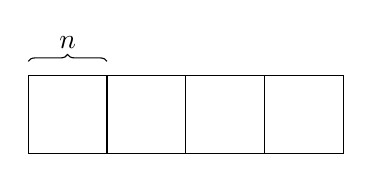
\begin{tikzpicture}
      % Frame
      \draw (0, 0) rectangle (1, 1);
      \draw (1, 0) rectangle (2, 1);
      \draw (2, 0) rectangle (3, 1);
      \draw (3, 0) rectangle (4, 1);

      % Brace
      \draw[decoration={brace,raise=5pt},decorate] (0,1) -- node[above=6pt] {$n$} (1,1);
    \end{tikzpicture}
    \caption{\footnotesize Free memory of size $4n$}
  \end{subfigure}
  \begin{subfigure}{.4\textwidth}
    \centering
    \begin{tikzpicture}
      % Background
      \fill[fill = grey] (0, 0) rectangle (3, 1) node[midway] {};
  
      % Frame
      \draw (0, 0) rectangle (1, 1) node[pos=.5] {$A$};
      \draw (1, 0) rectangle (3, 1) node[pos=.5] {$B$};
      \draw (3, 0) rectangle (4, 1);

      % Braces
      \draw[decoration={brace,raise=5pt},decorate] (0,1) -- node[above=6pt] {$n$} (1,1);
      \draw[decoration={brace,raise=5pt},decorate] (1,1) -- node[above=6pt] {$2n$} (3,1);
    \end{tikzpicture}
    \caption{\footnotesize Allocate $A$ and $B$}
  \end{subfigure}
  \vskip 1em
  \begin{subfigure}{.6\textwidth}
    \centering
    \begin{tikzpicture}
      % Background
      \fill[fill = grey] (1, 0) rectangle (3, 1) node[midway] {};
  
      % Frame
      \draw (0, 0) rectangle (1, 1);
      \draw (1, 0) rectangle (3, 1) node[pos=.5] {$B$};
      \draw (3, 0) rectangle (4, 1);
    \end{tikzpicture}
    \caption{\footnotesize Free $A$. Cannot fit another $B$ due to external fragmentation}
  \end{subfigure}
  \caption{Example of external fragmentation caused for allocation and deallocation order}
  \label{fig:external-frag-example}
\end{figure}  

Figure~\ref{fig:external-frag-example} shows this example, where the allocation and deallocation order causes a situation, in which we cannot allocate any more $B$ objects, even though we physically have the required amount of free space in memory. 

\begin{figure}[ht]
  \centering
  \begin{subfigure}{.4\textwidth}
    \centering
    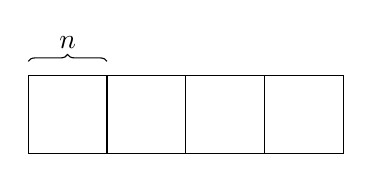
\begin{tikzpicture}
      % Frame
      \draw (0, 0) rectangle (1, 1);
      \draw (1, 0) rectangle (2, 1);
      \draw (2, 0) rectangle (3, 1);
      \draw (3, 0) rectangle (4, 1);

      % Brace
      \draw[decoration={brace,raise=5pt},decorate] (0,1) -- node[above=6pt] {$n$} (1,1);
    \end{tikzpicture}
    \caption{\footnotesize Free memory of size $4n$}
  \end{subfigure}
  \begin{subfigure}{.4\textwidth}
    \centering
    \begin{tikzpicture}
      % Background
      \fill[fill = grey] (0, 0) rectangle (3, 1) node[midway] {};
  
      % Frame
      \draw (0, 0) rectangle (2, 1) node[pos=.5] {$B$};
      \draw (2, 0) rectangle (3, 1) node[pos=.5] {$A$};
      \draw (3, 0) rectangle (4, 1);

      % Braces
      \draw[decoration={brace,raise=5pt},decorate] (0,1) -- node[above=6pt] {$2n$} (2,1);
      \draw[decoration={brace,raise=5pt},decorate] (2,1) -- node[above=6pt] {$n$} (3,1);
    \end{tikzpicture}
    \caption{\footnotesize Allocate $B$ and $A$}
  \end{subfigure}
  \vskip 1em
  \begin{subfigure}{.4\textwidth}
    \centering
    \begin{tikzpicture}
      % Background
      \fill[fill = grey] (0, 0) rectangle (2, 1) node[midway] {};
  
      % Frame
      \draw (0, 0) rectangle (2, 1) node[pos=.5] {$B$};
      \draw (2, 0) rectangle (3, 1);
      \draw (3, 0) rectangle (4, 1);
    \end{tikzpicture}
    \caption{\footnotesize Free $A$}
  \end{subfigure}
  \begin{subfigure}{.4\textwidth}
    \centering
    \begin{tikzpicture}
      % Background
      \fill[fill = grey] (0, 0) rectangle (4, 1) node[midway] {};
  
      % Frame
      \draw (0, 0) rectangle (2, 1) node[pos=.5] {$B$};
      \draw (2, 0) rectangle (4, 1) node[pos=.5] {$B$};
    \end{tikzpicture}
    \caption{\footnotesize Allocate another $B$}
  \end{subfigure}
  \caption{Example of avoiding external fragmentation using allocation and deallocation order}
  \label{fig:external-frag-example-cont}
\end{figure}  

Figure~\ref{fig:external-frag-example-cont} shows how changing allocation and deallocation order can combat external fragmentation.

\section{Memory Garbage}
\label{sec:memory-garbage}
A reversible computation should be garbage-free and as such it should be our goal to return the memory to its original state after program termination.

Traditionally, in non-reversible programming languages, freed memory blocks are simply re-added to the free-list during deallocation and no modification of the actual data stored in the block is performed, as it simply is overwritten when the block is used later on. In the reversible setting we must return the memory block to its original state after the block has been freed (e.g. zero-cleared), to uphold the time-invertible and two-directional computational model. Figure~\ref{fig:injective-garbage-in-out} illustrates how the output data (or garbage) of an injective function $f$ is the input to its inverse function $f'$.

In heap allocation layouts, we maintain one or more free-lists to keep track of free blocks during program execution, which are stored in memory, besides the heap representation itself. These free-lists can essentially be considered garbage and as such, they must also be returned to their original state after execution. Furthermore, the heap itself can also be considered garbage and if it grows during execution, it should also be returned to its original size.

\begin{figure}[ht]
  \centering
    \begin{tikzpicture}
      % lines
      \draw[-] (-1,1.75) node[left]{$in$} -- (9,1.75) node[right] {$in$};
      \draw[-] (2,1.25) -- (6,1.25);
      \draw[-] (2,0.75) -- (6,0.75);
      \draw[-] (2,0.25) -- (6,0.25);
      \draw[-] (-1,-0.5) node[left]{$out$} -- (9,-0.5) node[right] {$out$};
      \draw[-] (4,0.24) node[circle,fill,inner sep=1pt] {} -- (4,-0.5) node[circle,fill,inner sep=1pt] {};
      
      % boxes
      \draw[fill = white] (0, 0) rectangle (2, 2) node[pos=0.5] {\Large $f$};
      \draw[fill = white] (6, 0) rectangle (8, 2) node[pos=0.5] {\Large $f'$};
      \node[diamond, fill=white, draw] at (4,1.25) {\scriptsize $garbage$};
    \end{tikzpicture}
    \caption{The "garbage" output of an injective function $f$ is the input to its inverse function $f'$}
    \label{fig:injective-garbage-in-out}
\end{figure}

Returning the free-list(s) to their original states is a non-trivial matter, which is highly dependent on the heap layout and free-list design.~\citeauthor{ha:heap} introduced a dynamic memory manager which allowed heap allocation and deallocation, but without restoring the free-list to its original state in~\cite{ha:heap}.~\citeauthor{ha:heap} argue that an unrestored free-list can be considered harmless garbage in the sense that the free-list residing in memory after termination is equivalent to a restored free-list, as it contains the same blocks, but linked in a different order, depending on the order of allocation and deallocation operations performed during program execution. Figure~\ref{fig:equivalent-free-lists} illustrates how an inverse, injective function $f'$, whose non-inverse function $f$ computes something which modifies a given free lists, does not require the \textit{exact} output free list of $f$, but \textit{any} free list of same layout as input for the inverse function $f'$. The output free list of $f'$ will naturally be a further modified free list.

\begin{figure}[ht]
  \centering
  % 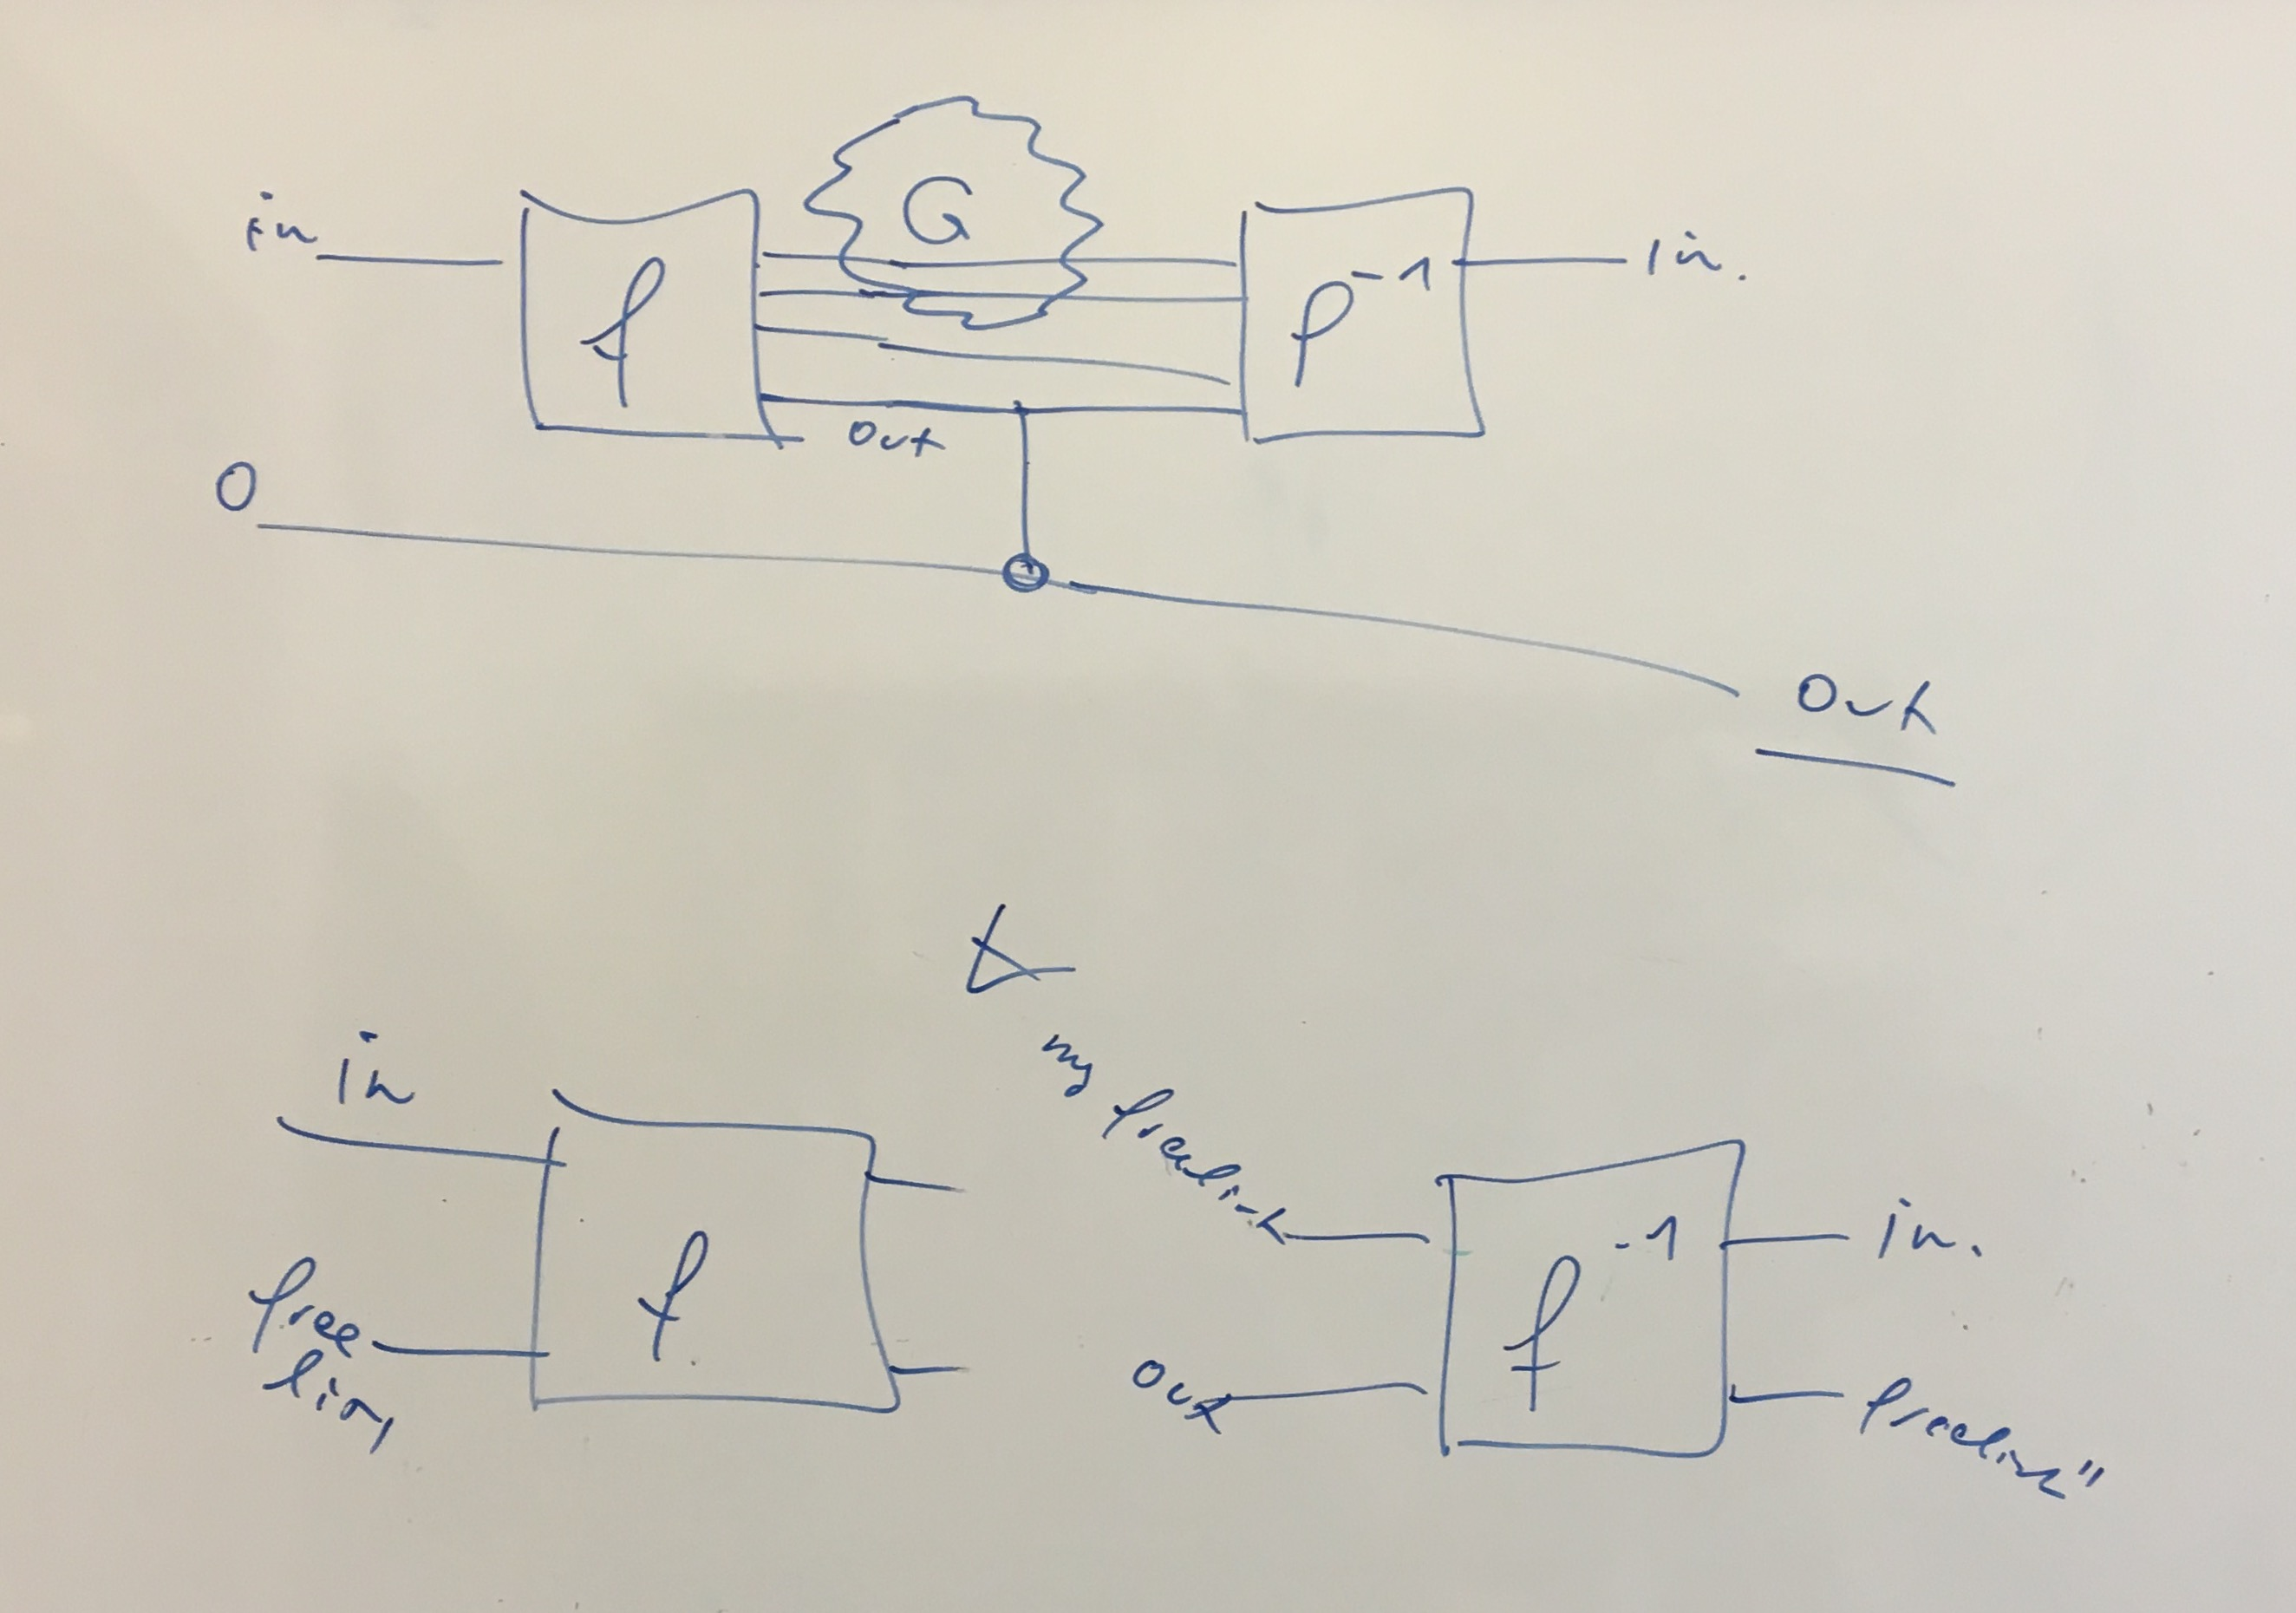
\includegraphics[width=0.7\textwidth]{garbage-classes}
  \begin{tikzpicture}
    % lines
    \draw[-] (-1,1.75) node[left]{$free\ list$} -- (2,1.75);
    \draw[-] (-1,0.25) node[left]{$in$} -- node[below] {$out$} (10,0.25) node[right] {$in$};
    \draw (7,1.75) .. controls (6,1.75) and (6,1.75) .. (6,2.75) node[above] {$\forall\ free\ lists$};
    \draw (2,1.75) .. controls (3,1.75) and (3,1.75) .. (3,2.75) node[above] {$free\ list'$};
    \draw[-] (9,1.75) -- (10,1.75) node[right]{$free\ list''$};
    
    % boxes
    \draw[fill = white] (0, 0) rectangle (2, 2) node[pos=0.5] {\Large $f$};
    \draw[fill = white] (7, 0) rectangle (9, 2) node[pos=0.5] {\Large $f'$};
  \end{tikzpicture}
  \caption{All free-lists are considered equivalent "garbage" in terms of injective functions}
  \label{fig:equivalent-free-lists}
\end{figure}

This intuitively leads to the question of garbage classification. In the reversible setting all functions are injective. Thus, given some $input_f$, in a reversible computation using heap allocation, the injective function $f$ produces some $output_f$ and some $garbage_f$ (e.g. garbage in form of storing data in the heap, so the free list changes, the heap grows, etc.). Its inverse function $f^{-1}$ must thus take $f$'s $output_f$ and $garbage_f$ as $input_{f^{-1}}$ to produce its output $output_{f^{-1}}$ which is $f$'s $input_f$. However, in the context of reversible heaps, we must consider all free-lists as of "equivalent garbage class" and thus freely substitutable with each other, as injective functions still can drastically change the block layout, free-list order, etc. during its execution in either direction. Figure~\ref{fig:equivalent-free-lists} shows how any free-list can be passed between a function $f$ and its inverse $f^{-1}$.


\section{Linearity and Reference Counting}
\label{sec:referencing}
% cite: http://home.pipeline.com/~hbaker1/Use1Var.html
Programming languages uses different approaches for storing and synchronizing variables and objects in memory. Typing \textit{linearity} is a distinction, which can reduce storage management and synchronization costs. %TODO: Cite here.

Reversible programming languages such as \textsc{Janus} and \textsc{Roopl} are linear in the sense that object and variable pointers cannot be copied and are only deleted during deallocation. Pointer copying greatly increases the flexibility of programming, especially in a reversible settings where zero-clearing is critical, at the cost of increased management in form of reference counting for e.g. objects. For variables, pointer copying is not particular interesting, nor would it add much flexibility as the values of a variable simply can be copied into statically-scoped local blocks. For objects however, tedious amounts of boilerplate work must be done if object $A$ and $B$ need to work on the same object $C$ and only one reference to each object is allowed.

\citeauthor{tm:refcounting} presented the reversible functional language \textsc{Rcfun} which used reference counting to allow multiple pointers to the same memory nodes as well as a translation from \textsc{Rcfun} into \textsc{Janus} in \cite{tm:refcounting}. In \textsc{Rcfun}, reference counting is used to manage and trace the number of pointer copies made by respectively incrementing and decrementing a \textit{reference count} stored in the memory node, whenever the original node pointer is copied or a copy pointer is deleted. For the presented heap manage, deletion of object nodes was only allowed when no references to a node remained.

In non-reversible languages, reference counting is also used in garbage collection by automatically deallocating unreachable objects and variables which contains no referencing. 


\section{Heap Manager Layouts}
\label{sec:heap-manager-layout}
Heap managers can be implemented in numerous ways. Different layouts yield advantages when allocating memory, finding a free block or when collecting garbage. As our goal is to construct a garbage-free heap manager, our finalized design should emphasize and reflect this objective in particular. Furthermore, we should attempt to allocate and deallocate memory as efficiently as possible, as merging and splitting of blocks is a non-trivial problem in a reversible setting and to avoid problematic fragmentation.

For the sake of simplicity, we will not consider the the issue of retrieving memory pages reversibly. A reversible operating system is a long-term dream of the reversible researcher and as reversible programming language designers, we assume that \rooplpp will be running in an environment, in which an operating system will be supplying memory pages and their mappings. As such, the following heap memory designs reflect this preliminary assumption, that we always can query the operating system for more memory. 

Historically, most object-oriented programming languages utilize a dynamic memory manager during program execution. In older, lower-level languages such as \textsc{C}, memory management is manual and allocation has to be stated explicitly and with the requested size through the \texttt{malloc} statement and deallocated using the \textbf{free} statement. Modern languages, such as \textsc{C\texttt{++}}, \textsc{Java} and \textsc{Python}, \textit{automagically} allocates and frees space for objects and variable-sized arrays by utilizing their dynamic memory manager and garbage collector to dispatch \textbf{malloc}- and \textbf{free}-like operations to the operating system and managing the obtained memory blocks in private heap(s)~\cite{wh:cpp_memory, bv:jvm, py:memory}. The heap layout of these managers vary from language to language and compiler to compiler.

Previous work on reversible heap manipulation has been done for reversible functional languages in~\cite{ha:heap, jsk:translation, tm:garbage}.

\citeauthor{ha:heap} presented a static heap structure consisting of \textsc{Lisp}-inspired constructor cells of fixed size and a single free list for the reversible function language \textsc{Rfun} in~\cite{ha:heap}. \citeauthor{tm:refcounting} presented an implementation in \textsc{Janus} of reversible reference counting under the assumption of \citeauthor{ha:heap}'s heap manager in~\cite{tm:refcounting}. Building on the previous work, \citeauthor{tm:garbage} later presented a reversible intermediate language \textsc{Ril} and an implementation in \textsc{Ril} of a reversible heap manager, which uses reference counting and hash-consing to achieve garbage collection in~\cite{tm:garbage}.

We do not consider reference counting or garbage collection in the layouts presented in the following sections, but we later show how the selected layout for \rooplpp is extended with reference counting in~\ref{sec:referencing-compilation}.

\subsection{Memory Pools}
\label{subsec:memory-pools}
The simplest heap layout we can design simple uses fixed-sized blocks. This design is also known as memory pools, as memory is allocated from "pools" of fixed-sized blocks regardless of the record size.
To model these pools of fixed-sized blocks, we simply use a linked-list of identically sized free block cells, which we maintain over execution.
While the fixed-block layout is simple and relatively easy in terms of implementation it is also largely uninteresting as it provides little to no options, besides sizing of the fixed-blocks, to combat fragmentation.

This layout comes with a few options in terms of the actual heap layout. If we only allow allocation of consecutive, adjacent free blocks, we should keep the free list sorted. If the free list is not sorted, and we have to allocate an object which requires $n$ blocks, we have to iterate the free list $n^2$ times in the worst case to find a chain of consecutive blocks large enough to fit the object. The sorting part itself is non-trivial matter. Furthermore, we need some overhead storage inside the object to contains the references of the blocks occupied by the object, or some other structure which can be used when deallocating the object and returning all the blocks to the free list. If we allow allocation of non-consecutive blocks, larger amounts of book-keeping is required as we need to store knowledge of when and where the object is split.

Figures~\ref{fig:external-frag-example} and~\ref{fig:external-frag-example} from earlier in this chapter, in section~\ref{subsec:external-fragmentation} on page~\pageref{fig:external-frag-example} illustrates examples with consecutive, fixed-sized block allocation. 


\subsection{One Heap Per Record Size}
\label{subsec:one-heap-per-record-size}
Instead of allocating space for objects from a single free list and heap, we could design an approach which uses one heap per record size. The respective classes and their sizes are easily identified during compile time from which the amount of heaps and free list will be initialized. This means the layout is very dynamic and potentially can change drastically in terms of the amount of heaps utilized depending on the input program. 

\begin{figure}[ht]
  \centering
  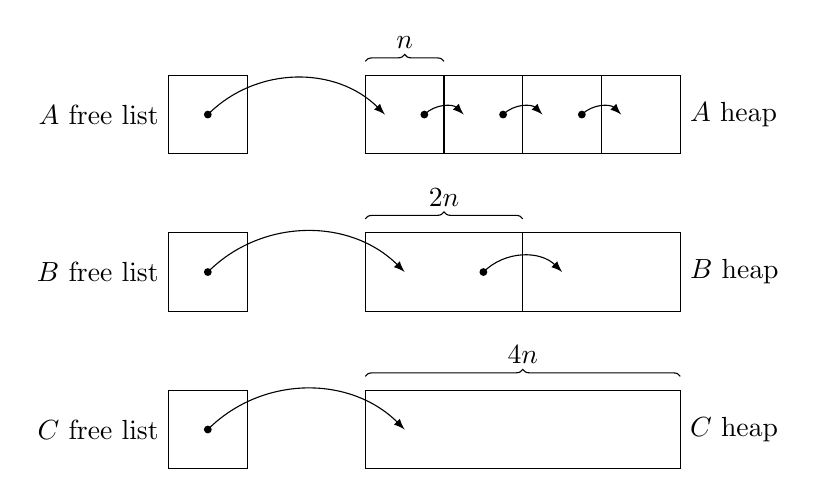
\begin{tikzpicture}
    % Heaps
    \draw[step=1cm] (0,4) grid (4,5);
    \node[right] at (4,4.5) {$A$ heap}; 
    \draw (0,2) rectangle (2,3) rectangle node[right, xshift=1cm] {$B$ heap} (4,2);
    \draw (0,0) rectangle node[right, xshift=2cm] {$C$ heap} (4,1);

    % Free lists
    \draw (-2.5, 4) rectangle node[left, xshift=-0.5cm] {$A$ free list} (-1.5, 5);
    \draw (-2.5, 2) rectangle node[left, xshift=-0.5cm] {$B$ free list} (-1.5, 3);
    \draw (-2.5, 0) rectangle node[left, xshift=-0.5cm] {$C$ free list} (-1.5, 1);
    
    % Arrow for 1st heap pair
    \node[circle,fill,inner sep=1pt] at (-2, 4.5) {};
    \draw[-latex] (-2, 4.5) to[out=45, in=135] (0.25, 4.5);
    \node[circle,fill,inner sep=1pt] at (0.75, 4.5) {};
    \draw[-latex] (0.75, 4.5) to[out=45, in=135] (1.25, 4.5);
    \node[circle,fill,inner sep=1pt] at (1.75, 4.5) {};
    \draw[-latex] (1.75, 4.5) to[out=45, in=135] (2.25, 4.5);
    \node[circle,fill,inner sep=1pt] at (2.75, 4.5) {};
    \draw[-latex] (2.75, 4.5) to[out=45, in=135] (3.25, 4.5);

    % Arrow for 2nd heap pair
    \node[circle,fill,inner sep=1pt] at (-2, 2.5) {};
    \draw[-latex] (-2, 2.5) to[out=45, in=135] (0.5, 2.5);
    \node[circle,fill,inner sep=1pt] at (1.5, 2.5) {};
    \draw[-latex] (1.5, 2.5) to[out=45, in=135] (2.5, 2.5);

    % Arrow for 3rd heap pair
    \node[circle,fill,inner sep=1pt] at (-2, 0.5) {};
    \draw[-latex] (-2, 0.5) to[out=45, in=135] (0.5, 0.5);

    % Braces
    \draw[decoration={brace,raise=5pt},decorate] (0,1) -- node[above=6pt] {$4n$} (4,1);
    \draw[decoration={brace,raise=5pt},decorate] (0,3) -- node[above=6pt] {$2n$} (2,3);
    \draw[decoration={brace,raise=5pt},decorate] (0,5) -- node[above=6pt] {$n$} (1,5);
  \end{tikzpicture}
  \caption{Memory layout using one heap per record size}
  \label{fig:one-heap-per-record-size}
\end{figure}

Figure~\ref{fig:one-heap-per-record-size} illustrates three heaps with respective free lists for three classes $A$, $B$ and $C$ of size $n$, $2n$ and $4n$. Each heap is represented as a simple linked list with the free list simply being a pointer to the first free block in the heap. 

The advantage of this approach would be effective elimination of internal and external fragmentation, as each heap fits their targeted record perfectly, making each allocation and deallocation tailored to the size of the record obtained from a static analysis during compilation, resulting in no over-allocation and no unusable chunks of freed memory appearing during varying deallocation order. Implementation-wise, allocation of an object of a given class simply becomes the task of popping the head of the respective free list, which easily can be determined at compile time. The inverse deallocation is simply added a new head to the free list.

Listing~\ref{lst:one-heap-per-record-size} outlines the allocation algorithm for this layout written in extended \textsc{Janus} from~\cite{ty:ejanus}. We assume that the heads of the free lists are stored in a single array primitive, such that the free list for records of size $n$ are indexed at $n-2$ and $n > 2$ (as every record needs some overhead) and that we have heaps for continuous size range with no gaps. To maintain reversibility we only allow allocation from the head of the free list.

The algorithm consists of an entry point named \textbf{malloc} and a recursion body named \textbf{malloc1}. Given a zero-cleared pointer \texttt{p}, the size of the object we are allocating \texttt{osize} and the freelists array primitive, the recursion body is called after initializing a \texttt{counter}, which is an index into the free lists array and a counter size, \texttt{csize}, which is the block size of the current free list the \texttt{counter} is indexed in. The recursion body first updates the free list index until we find a free list greater or equal to the size of the object we are allocating. Once found, we enter the next conditional, which searches for a free lists with a free block that is greater or equal to the size of our object. Once such a free list has been found, the head of the free list is simply popped and the next block is set as the new head.

\begin{lstlisting}[caption={Allocation algorithm for one heap per record size implemented in extended Janus.}, language=janus, style=basic, label={lst:one-heap-per-record-size}]
  procedure malloc(int p, int osize, int freelists[])
    local int counter = 0
    local int csize = 2
    call malloc1(p, osize, freelists, counter, csize)
    delocal int csize = 2
    delocal int counter = 0

  procedure malloc1(int p, int osize, int freelists[], int counter, int csize)
    if (csize < osize) then
        counter += 1
        csize += 1
        call malloc1(p, osize, freelists, counter, csize) 
        csize -= 1
        counter -= 1
    else
        if freelists[counter] != 0 then
            p += freelists[counter]
            freelists[counter] -= p

            // Swap head of free list with p's next block
            freelists[counter] ^= M(p)
            M(p) ^= freelists[counter]
            freelists[counter] ^= M(p)
        else
            counter += 1
            csize += 1
            call malloc1(p, osize, freelists, counter, csize)
            csize -= 1
            counter -= 1
        fi freelists[counter] = 0 || p != freelists[counter]
    fi csize < osize   
\end{lstlisting}

The obvious disadvantage to this layout is the amount of book-keeping and workload associated with growing and shrinking a heap and its neighbours, in case the program requests additional memory from the operating system. In real world object-oriented programming, most classes features a small number of fields, very rarely more than 16. As such, multiple heaps of same record size would exist, which intuitively seems inefficient. 

Additional, small helper classes would spawn additional heaps and additional book-work, making the encapsulation concept of OOP rather unattractive, for the optimization-oriented reversible programmer. 

Finally, while internal and external fragmentation is effectively eliminated, we are left with additional and considerable amounts of garbage in forms of all the heaps and free lists initialized in memory. If two record types only differ one word in size, two heaps would be initialized. Each heap intuitively needs to be initialized with a chunk of memory from the underlying operating system such that objects can be allocated on their respective heaps, regardless of the number of times the heap is used during program execution. This is an obvious space requirement increase over the previously presented layout, and on average, the amount of required memory for a program compiled using this approach would probably be larger, than some of the following layouts, due to unoptimized heap utilization and sharing.


\subsection{One Heap Per Power-Of-Two}
\label{subsec:one-heap-per-power-of-two}
To address the issues of the previous heap manager layout, we can optimize the amounts of heaps required by introducing a relatively small amount of internal fragmentation. Instead of having a heap per record size, we could instead have a heap per power-of-two. Records would be stored in the heap closest to their respective size and as such, we reduce the number of heaps needed, as many different records can be stored in the same heap. Records of size $5$, $6$, $7$ and $8$ would in the former layout be stored in four different heaps, where they would be stored in a single heap using this layout. Figure~\ref{fig:one-heap-per-power-of-two} illustrates the free lists and heaps up to $n^m$. 

\begin{figure}[ht]
  \centering
  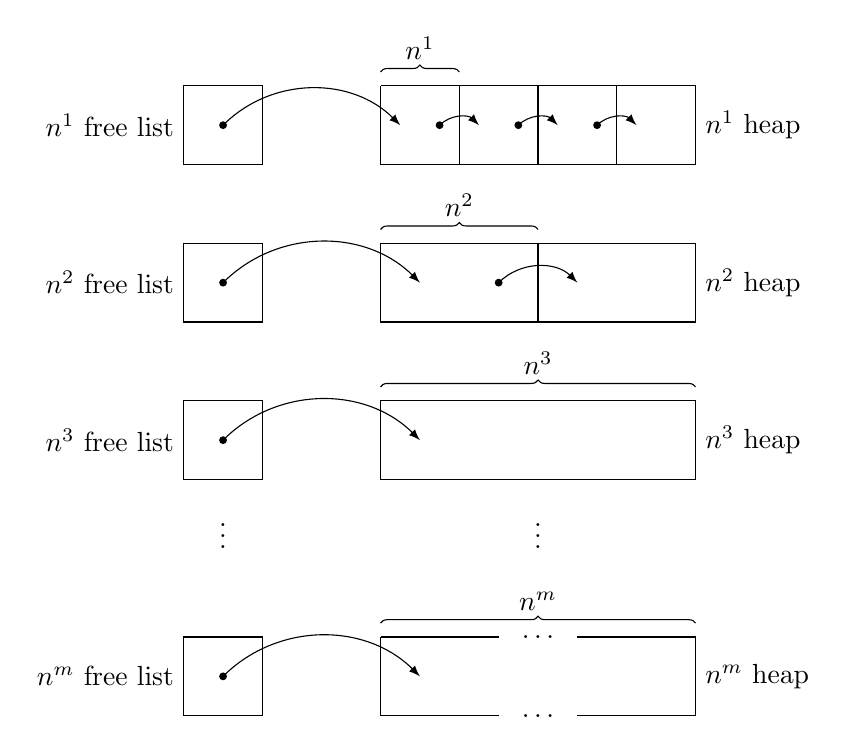
\begin{tikzpicture}
    % Heaps
    \draw[step=1cm] (0,4) grid (4,5);
    \node[right] at (4,4.5) {$n^1$ heap}; 
    \draw (0,2) rectangle (2,3) rectangle node[right, xshift=1cm] {$n^2$ heap} (4,2);
    \draw (0,0) rectangle node[right, xshift=2cm] {$n^3$ heap} (4,1);

    \draw (0,-3) -- (0, -2);
    \draw (0,-3) -- (1.5, -3);
    \draw (0,-2) -- (1.5, -2);
    \draw (2.5,-3) -- (4, -3);
    \draw (2.5,-2) -- (4, -2);
    \draw (4,-3) -- (4, -2);
    \node[right] at (4,-2.5) {$n^m$ heap};  

    % Free lists
    \draw (-2.5, 4) rectangle node[left, xshift=-0.5cm] {$n^1$ free list} (-1.5, 5);
    \draw (-2.5, 2) rectangle node[left, xshift=-0.5cm] {$n^2$ free list} (-1.5, 3);
    \draw (-2.5, 0) rectangle node[left, xshift=-0.5cm] {$n^3$ free list} (-1.5, 1);
    \draw (-2.5, -3) rectangle node[left, xshift=-0.5cm] {$n^m$ free list} (-1.5, -2);
    
    % Arrow for 1st heap pair
    \node[circle,fill,inner sep=1pt] at (-2, 4.5) {};
    \draw[-latex] (-2, 4.5) to[out=45, in=135] (0.25, 4.5);
    \node[circle,fill,inner sep=1pt] at (0.75, 4.5) {};
    \draw[-latex] (0.75, 4.5) to[out=45, in=135] (1.25, 4.5);
    \node[circle,fill,inner sep=1pt] at (1.75, 4.5) {};
    \draw[-latex] (1.75, 4.5) to[out=45, in=135] (2.25, 4.5);
    \node[circle,fill,inner sep=1pt] at (2.75, 4.5) {};
    \draw[-latex] (2.75, 4.5) to[out=45, in=135] (3.25, 4.5);

    % Arrow for 2nd heap pair
    \node[circle,fill,inner sep=1pt] at (-2, 2.5) {};
    \draw[-latex] (-2, 2.5) to[out=45, in=135] (0.5, 2.5);
    \node[circle,fill,inner sep=1pt] at (1.5, 2.5) {};
    \draw[-latex] (1.5, 2.5) to[out=45, in=135] (2.5, 2.5);

    % Arrow for 3rd heap pair
    \node[circle,fill,inner sep=1pt] at (-2, 0.5) {};
    \draw[-latex] (-2, 0.5) to[out=45, in=135] (0.5, 0.5);

    % Arrow for 4th heap pair
    \node[circle,fill,inner sep=1pt] at (-2, -2.5) {};
    \draw[-latex] (-2, -2.5) to[out=45, in=135] (0.5, -2.5);

    % Braces
    \draw[decoration={brace,raise=5pt},decorate] (0,5) -- node[above=6pt] {$n^1$} (1,5);
    \draw[decoration={brace,raise=5pt},decorate] (0,3) -- node[above=6pt] {$n^2$} (2,3);
    \draw[decoration={brace,raise=5pt},decorate] (0,1) -- node[above=6pt] {$n^3$} (4,1);
    \draw[decoration={brace,raise=5pt},decorate] (0,-2) -- node[above=6pt] {$n^m$} (4,-2);

    % Dots
    \node[above] at (-2, -1) {$\vdots$};
    \node[above] at (2, -1) {$\vdots$};
    \node[] at (2, -2) {$\dots$};
    \node[] at (2, -3) {$\dots$};
  \end{tikzpicture}
  \caption{Memory layout using one heap per power-of-two}
  \label{fig:one-heap-per-power-of-two}
\end{figure}

Internal fragmentation does become a problem for very large records, as blocks only are of size $2^n$. An object of size $65$ would fit on a $128$ sized block, resulting in considerable amounts of wasted memory space in form of internal fragmentation. However, in the real world, most records are small and allocation of records causing this much amount of fragmentation is an unlikely scenario. To avoid large amounts of internal fragmentation building up when allocating large records, we could allocate space for large objects using smaller blocks. If a record exceeds some limit, which has been determined the cutoff point, one kilobyte for an example, we could split it into $\sqrt{n}$ sized chunks and use blocks of that size instead. This would reduce the amount of internal fragmentation at the cost of increased book-keeping.
For smaller records, very minimal amounts of internal fragmentation appears. 

The number of heaps needed for a computation can be determined at compile time by finding the smallest and largest record sizes and ensuring we have heaps to fit these effectively. The allocation process consists of determining the closest $2^n$ to the size of the record we are allocating and then simply popping the head of the respective free list.

Listing~\ref{lst:one-heap-per-power-of-two} shows a modified \textbf{malloc1} recursion body for the power-of-two approach. Once again, we assume our free lists array contains the heads of each free list, such that index $n$ is the head of the free list of size $2^{n+1}$. Instead of incrementing the counter size by one as in the the former layout algorithm we not double it, using the shown procedure. Besides this change, the algorithm remains unchanged and still assume each heap has been initialized along with the free lists.\\

\begin{lstlisting}[caption={Allocation algorithm for one heap per power of two implemented in extended Janus.}, language=janus, style=basic, label={lst:one-heap-per-power-of-two}]
  procedure double(int target)
    local int current = target
    target += current
    delocal int current = target / 2

  procedure malloc1(int p, int osize, int freelists[], int counter, int csize)
    if (csize < osize) then
        counter += 1
        call double(csize)
        call malloc1(p, osize, freelists, counter, csize) 
        uncall double(csize)
        counter -= 1
    else
        if freelists[counter] != 0 then
            p += freelists[counter]
            freelists[counter] -= p

            // Swap head of free list with p's next block
            freelists[counter] ^= M(p)
            M(p) ^= freelists[counter]
            freelists[counter] ^= M(p)
        else
            counter += 1
            call double(csize)
            call malloc1(p, osize, freelists, counter, csize)
            uncall double(csize)
            counter -= 1
        fi freelists[counter] = 0 || p != freelists[counter]
    fi csize < osize   
\end{lstlisting}


\subsection{Shared Heap, Record Size-Specific Free Lists}
\label{subsec:shared-heap}
A natural proposal, considering the disadvantages of the previously presented design, would be using a shared heap instead of record-specific heaps. 
This way, we ensure minimal fragmentation when allocating and freeing as the different free lists ensures that allocation of an object wastes as little memory as possible. By only keeping one heap, we eliminate the growth/shrinking issues of the multiple heap layout. 

There is, however, still a considerable amount of book-keeping involved in maintaining multiple free-lists. Having mixed-sized blocks in a single heap is also a task which might prove difficult to maintain in a reversible setting. How initialization and destruction of said heap should work is not clear. As with the multiple heap version of this layout, we are still left with the issues surrounding two records which only differs one word in size. In the former layout, two heaps were required to store records of these types. In this layout, we need to store two block sizes in our heap to allocated these records, with no internal fragmentation. We could allow these objects to be allocated on similarly-sized blocks, if we round the calculated class sizes up to, say, a power of two. We would essentially have a shared heap, power-of-two-specific free lists layout.

\begin{figure}[ht]
  \centering
  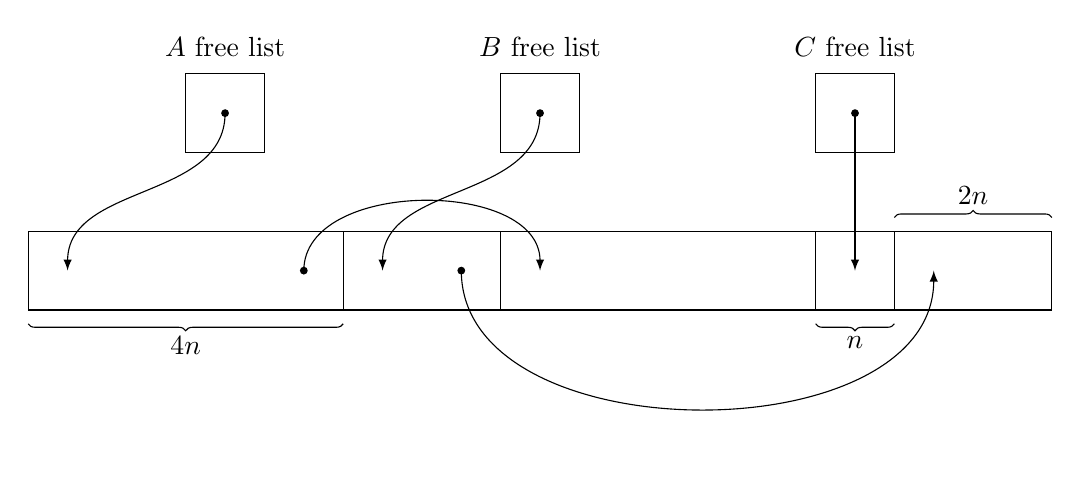
\begin{tikzpicture}
    % Heap
    \draw (0, 0) rectangle (4, 1);
    \draw (4, 0) rectangle (6, 1);
    \draw (6, 0) rectangle (10, 1);
    \draw (10, 0) rectangle (11, 1);
    \draw (11, 0) rectangle (13, 1);

    % Free lists
    \draw (2, 2) rectangle (3, 3) node[midway, above, yshift=0.6cm] {$A$ free list}; 
    \draw (6, 2) rectangle (7, 3) node[midway, above, yshift=0.6cm] {$B$ free list};
    \draw (10, 2) rectangle (11, 3) node[midway, above, yshift=0.6cm] {$C$ free list};

    % Arrows 1st heap
    \node[circle,fill,inner sep=1pt] at (2.5, 2.5) {};
    \draw[-latex] (2.5, 2.5) to[out=270, in=90] (0.5, 0.5);

    \node[circle,fill,inner sep=1pt] at (3.5, 0.5) {};
    \draw[-latex] (3.5, 0.5) to[out=90, in=90] (6.5, 0.5);

    % Arrows 2nd heap
    \node[circle,fill,inner sep=1pt] at (6.5, 2.5) {};
    \draw[-latex] (6.5, 2.5) to[out=270, in=90] (4.5, 0.5);

    \node[circle,fill,inner sep=1pt] at (5.5, 0.5) {};
    \draw[-latex] (5.5, 0.5) to[out=-90, in=-90] (11.5, 0.5);

    % Arrows 3rd heap
    \node[circle,fill,inner sep=1pt] at (10.5, 2.5) {};
    \draw[-latex] (10.5, 2.5) to[out=270, in=90] (10.5, 0.5);

    % Braces
    \draw[decoration={brace, mirror, raise=5pt},decorate] (0,0) -- node[below=6pt] {$4n$} (4,0);
    \draw[decoration={brace, mirror, raise=5pt},decorate] (10,0) -- node[below=6pt] {$n$} (11,0);
    \draw[decoration={brace, raise=5pt},decorate] (11,1) -- node[above=6pt] {$2n$} (13,1);
  \end{tikzpicture}
  \caption{Record size-specific free lists on a shared heap}
  \label{fig:shared-heap}
\end{figure}

As the only change in this design are the heaps themselves, the allocation process remains unchanged from the one presented in listing~\ref{lst:one-heap-per-record-size}. Figure~\ref{fig:shared-heap} visualizes the shared heap and the free lists of this layout.


\subsection{Buddy Memory}
\label{subsec:buddy-memory}
The Buddy Memory layout utilizes blocks of variable-sizes of the power-of-two, typically with one free list per power-of-two using a shared heap. When allocating an object of size $m$, we simply check the free lists for a free block of size $n$, where $n \geq m$. Is such a block found and if $n > m$, we split the block into two halves recursively, until we obtain the smallest block capable of storing $m$. When deallocating a block of size $m$, do the action described above in reverse, thus merging the blocks again, where possible.

\begin{figure}[ht]
  \centering
  \begin{subfigure}{.5\textwidth}
    \centering
    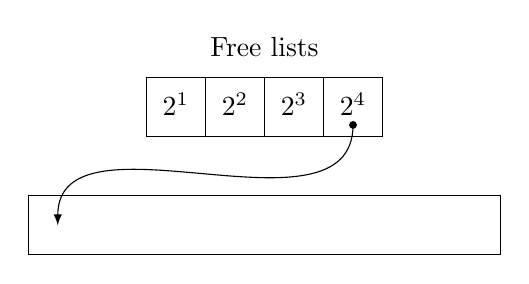
\begin{tikzpicture}[scale=0.75]
      % Boxes
      \draw[step=1] (2,2) grid (6,3);
      \draw (0,0) rectangle (8, 1);

      % Labels
      \node[above] at (4, 3.2) {Free lists}; 
      \node[above] at (2.5, 2.2) {$2^1$}; 
      \node[above] at (3.5, 2.2) {$2^2$}; 
      \node[above] at (4.5, 2.2) {$2^3$}; 
      \node[above] at (5.5, 2.2) {$2^4$}; 
      
      % Arrows
      \node[circle,fill,inner sep=1pt] at (5.5, 2.2) {};
      \draw[-latex] (5.5, 2.2) to[out=270, in=90] (0.5, 0.5);
    \end{tikzpicture}
    \caption{\footnotesize Initial memory block}
  \end{subfigure}%
  \begin{subfigure}{.5\textwidth}
    \centering
    \begin{tikzpicture}[scale=0.75]
      % Fills
      \draw[fill=grey] (7,0) rectangle (8,1);

      % Boxes
      \draw[step=1] (2,2) grid (6,3);
      \draw (0,0) rectangle (8, 1);

      % Labels
      \node[above] at (4, 3.2) {Free lists}; 
      \node[above] at (2.5, 2.2) {$2^1$}; 
      \node[above] at (3.5, 2.2) {$2^2$}; 
      \node[above] at (4.5, 2.2) {$2^3$}; 
      \node[above] at (5.5, 2.2) {$2^4$}; 

      % Lines
      \draw (4,0) -- (4, 1);
      \draw (6,0) -- (6, 1);
      \draw (7,0) -- (7, 1);
      
      % Arrows
      \node[circle,fill,inner sep=1pt] at (4.5, 2.2) {};
      \draw[-latex] (4.5, 2.2) to[out=270, in=90] (0.5, 0.5);

      \node[circle,fill,inner sep=1pt] at (3.5, 2.2) {};
      \draw[-latex] (3.5, 2.2) to[out=270, in=90] (4.5, 0.5);

      \node[circle,fill,inner sep=1pt] at (2.5, 2.2) {};
      \draw[-latex] (2.5, 2.2) to[out=270, in=90] (6.5, 0.5);
    \end{tikzpicture}
    \caption{\footnotesize Allocate an object of size $2^1$}
  \end{subfigure}%
  \vskip 1em
  \begin{subfigure}{.5\textwidth}
    \centering
    \begin{tikzpicture}[scale=0.75]
      % Fills
      \draw[fill=grey] (7,0) rectangle (8,1);
      \draw[fill=grey] (0,0) rectangle (4,1);

      % Boxes
      \draw[step=1] (2,2) grid (6,3);
      \draw (0,0) rectangle (8, 1);

      % Labels
      \node[above] at (4, 3.2) {Free lists}; 
      \node[above] at (2.5, 2.2) {$2^1$}; 
      \node[above] at (3.5, 2.2) {$2^2$}; 
      \node[above] at (4.5, 2.2) {$2^3$}; 
      \node[above] at (5.5, 2.2) {$2^4$}; 

      % Lines
      \draw (4,0) -- (4, 1);
      \draw (6,0) -- (6, 1);
      \draw (7,0) -- (7, 1);
      
      % Arrows
      \node[circle,fill,inner sep=1pt] at (3.5, 2.2) {};
      \draw[-latex] (3.5, 2.2) to[out=270, in=90] (4.5, 0.5);

      \node[circle,fill,inner sep=1pt] at (2.5, 2.2) {};
      \draw[-latex] (2.5, 2.2) to[out=270, in=90] (6.5, 0.5);
    \end{tikzpicture}
    \caption{\footnotesize Allocate an object of size $2^3$}
  \end{subfigure}%
  \begin{subfigure}{.5\textwidth}
    \centering
    \begin{tikzpicture}[scale=0.75]
      % Fills
      \draw[fill=grey] (7,0) rectangle (8,1);
      \draw[fill=grey] (0,0) rectangle (4,1);
      \draw[fill=grey] (4,0) rectangle (6,1);

      % Boxes
      \draw[step=1] (2,2) grid (6,3);
      \draw (0,0) rectangle (8, 1);

      % Labels
      \node[above] at (4, 3.2) {Free lists}; 
      \node[above] at (2.5, 2.2) {$2^1$}; 
      \node[above] at (3.5, 2.2) {$2^2$}; 
      \node[above] at (4.5, 2.2) {$2^3$}; 
      \node[above] at (5.5, 2.2) {$2^4$}; 

      % Lines
      \draw (4,0) -- (4, 1);
      \draw (6,0) -- (6, 1);
      \draw (7,0) -- (7, 1);
      
      % Arrows
      \node[circle,fill,inner sep=1pt] at (2.5, 2.2) {};
      \draw[-latex] (2.5, 2.2) to[out=270, in=90] (6.5, 0.5);
    \end{tikzpicture}
    \caption{\footnotesize Allocate an object of size $2^2$}
  \end{subfigure}%
  \caption{Buddy Memory block allocation example}
  \label{fig:buddy-memory-block-splitting}
\end{figure}

Figure~\ref{fig:buddy-memory-block-splitting} illustrates an example of block splitting during allocation in the buddy system. Originally, one block of free memory is available. When allocation a record three factors smaller than the original block, three splits occurs. 

This layout is somewhat of a middle ground between the previous three designs, addressing a number of problems found in these. The Buddy Memory layout uses a single heap for all record-types, thus eliminating the problems related to moving adjacent heaps reversibly in a multi-heap layout. To optimize the problems around initializing a usable amount of variable-sized blocks in a shared heap, we simply initialize one large block in the buddy system, which we will split into smaller parts during execution.

The only drawback from this layout is the amount of internal fragmentation. As we only allocate blocks of a power-of-two size, substantial internal fragmentation follows when allocating large records, i.e. a allocating a block of size 128 for a record of size 65. However, as most real world programs uses much smaller sized records, we do not consider this a very frequent scenario. As discussed in section~\ref{subsec:one-heap-per-power-of-two}, we would split large records into chunks of $\sqrt{n}$ at the cost of additional book-keeping.

Implementation-wise, this design would require doubling and halving of numbers related to the power-of-two. This action translates well into the reversible setting, as a simply bit-shifting directly gives us the desired result.

\begin{lstlisting}[caption={The Buddy Memory algorithm implemented in extended Janus.}, language=janus, style=basic, label={lst:buddy-memory}]
  procedure malloc1(int p, int osize, int freelists[], int counter, int csize, int next_block[])
    if (csize < osize) then
        counter += 1
        call double(csize)
        call malloc1(p, osize, freelists, counter, csize) 
        uncall double(csize)
        counter -= 1
    else
        if freelists[counter] != 0 then
            p += freelists[counter]
            freelists[counter] -= p

            // Swap head of free list with p's next block
            freelists[counter] ^= M(p)
            M(p) ^= freelists[counter]
            freelists[counter] ^= M(p)
        else
            counter += 1
            call double(csize)
            call malloc1(p, osize, freelists, counter, csize)
            uncall double(csize)
            counter -= 1
            freelists[counter] += p
            p += csize
        fi freelists[counter] = 0 || p - csize != freelists[counter]
    fi csize < osize   
\end{lstlisting}

Listing~\ref{lst:buddy-memory} shows the buddy memory algorithm implemented in the extended Janus variant with local blocks from~\cite{ty:ejanus}. For simplification in object sizes are rounded to the nearest power-of-two during compile-time and we only allow allocations using the heads of the free lists. The algorithm extends on the one heap per power-of-two algorithm presented in listing~\ref{lst:one-heap-per-power-of-two}, page~\pageref{lst:one-heap-per-power-of-two}.
The body of the allocation function is still executed recursively until a free list for a $2^n$ larger than the size of the object has been found. Once found, we continue searching until we have found a non-empty free list. If the non-empty free list for a $2^n$ larger than the object is found, the head of the list is popped and the popped block is split recursively, until a block the desired size is obtained. Throughout the splitting process, empty free lists are updated when a larger free block is split into a block which fits into those lists. 



\newpage

\chapter{Compilation}
\label{chp:compilation}
%TODO: Revise chapter intro
The following chapter will present the considerations and designs for the reversible heap manager and the schemes used in the process of translating \rooplpp to the reversible low-level machine language \textsc{PISA}.

\section{The \textsc{Roopl} to \textsc{Pisa} compiler}
\label{sec:roopl-to-pisa-compiler}
% TODO: Write section

\section{\rooplpp Memory Layout}
\label{sec:rooplpp-memory-layout}
\rooplpp builds upon its predecessor's memory layout with dynamic memory management. The reversible Buddy Memory heap layout presented in section~\ref{sec:buddy-memory} is utilized in \rooplpp as it is an interesting layout, naturally translates into a reversible setting with one simple restriction (i.e only blocks which are heads of their respectable free lists are allocatable) and since its only drawback is dismissible in most real world scenarios.

Figure~\ref{fig:memory-layout} shows the full layout of a \rooplpp program stored in memory.

\begin{itemize}
    \item As with \textsc{Roopl}, the static storage segment contains load-time labelled \inst{data} instructions, initialized with virtual function tables and other static data needed by the translated program.

    \item The program segment is stored right after the static storage and contains the translate \rooplpp program instructions.

    \item The free lists maintained by the Buddy Memory heap layout is placed right after the program segment, with the \textit{free list pointer} $flp$ pointing at the first free list. The free lists are simple the address to the first block of its respective size. The free lists are stores such that the free list at address $flp + i$ corresponds to the free list of size $2^{i+1}$.   

    \item The heap begins directly following the free lists. Its beginning is marked by the \textit{heap pointer} $(hp)$. 

    \item Unlike in \textsc{Roopl}, where the stack grows upwards, the \rooplpp stack grows downwards and is begins at address $p$. The stack remains a LIFO structure, analogously to \textsc{Roopl}.
\end{itemize}

As denoted in the previous section, we assume an underlying reversible operating system providing us with additional memory when needed. With no real way of simulating this, the \rooplpp compiler places the stack at a fixed address $p$ and sets one free block in the largest $2^n$ free list initially. The number of free lists and the address $p$ is configurable in the source code, but is defaulted to $10$ free lists, meaning initially one block of size $1024$ is available and the stack is placed at address $2048$.

In traditional compilers, the heap pointer usually points to the end of the heap. For reasons stated above, we never grow the heap as we start with a heap of fixed size. As such, the heap pointer simply points to the beginning of the heap.

\begin{figure}[ht]
    \centering
    
    \begin{tikzpicture}
        \fill[fill = grey] (0, 0) rectangle (2.5, 3) node[midway] {Static Data};
        \fill[fill = darkgrey] (2.5, 0) rectangle (5, 3) node[midway] {Program};
        \fill[fill = grey] (5, 0) rectangle (7, 3) node[midway] {Free lists};
        \fill[fill = grey] (7, 0) rectangle (8.5, 3) node[midway] {Heap};
        \fill[fill = grey] (12.5, 0) rectangle (14, 3) node[midway] {Stack}; 
        
        \draw (0, 0) -- (15, 0);
        \draw (0, 3) -- (15, 3);
        \draw (0, 0) -- (0, 3);
        \draw (15, 0) -- (15, 3);
        \draw (2.5, 0) -- (2.5, 3);
        \draw (5, 0) -- (5, 3); 
        \draw (7, 0) -- (7, 3);
        \draw (14, 0) -- (14, 3); 
        \draw[dashed] (8.5, 0) -- (8.5, 3); 
        \draw[dashed] (12.5, 0) -- (12.5, 3);   
    
        \node at (10.5, 2.5) {(unused memory)};
        \node at (0, -.3) {$0$};
        \node at (5, -.3) {$flp$};
        \node at (7, -.3) {$hp$};
        \node at (14, -.3) {$p$};
        \node at (12.5, -.3) {$sp$};
        \node at (15, -.3) {$2^{31} - 1$};
        \node at (7.5, -1) {$\longleftarrow$ Address Space $\longrightarrow$};

        \draw[arrow, dashed] (8.5, 1.5) -- (10.1, 1.5);
        \node at (9.4, 1.2) {\scriptsize{\textit{heap grows}}};

        \draw[arrow, dashed] (12.5, 1.5) -- (10.9, 1.5); 
        \node at (11.6, 1.2) {\scriptsize{\textit{stack grows}}};
    \end{tikzpicture}
    
    \caption{Memory layout of a \rooplpp program}
    \label{fig:memory-layout}
\end{figure}

\section{Inherited \textsc{Roopl} features}
As mentioned, a number of features from \textsc{Roopl} carries over in \rooplpp.

The dynamic dispatching mechanism presented in~\cite{th:roopl} is inherited. As such, the invocation of a method implementation is based on the type of the object at run time. Virtual function tables are still the implementation strategy used in the dynamic dispatching implementation.

Evaluation of expressions and control flow remains unchanged. 

For completeness, object blocks are included and still stack allocated as their life time is limited to the scope of their block and the dynamic allocation process is quite expensive in terms of register pressure and number of instructions compared to the stack allocated method presented implemented in the \textsc{Roopl} compiler.

The object layout remains unchanged (\textit{for now, until reference counting is added}) and is shown in figure~\ref{fig:object-layout}

\begin{figure}[h]
    \centering
    
    \begin{subfigure}[t]{.32\textwidth}
        \vskip 0pt
        \centering
        \begin{tikzpicture}
            \draw[dashed] (0, 1.5) -- (0, 2);
            \draw[dashed] (3, 1.5) -- (3, 2);
            \filldraw[fill = grey, draw = black] (0, 1) rectangle (3, 1.5) node[midway] {addr(vtable)};
            \filldraw[fill = darkgrey, draw = black] (0, .5) rectangle (3, 1) node[midway] {x};
            \filldraw[fill = grey, draw = black] (0, 0) rectangle (3, .5) node[midway] {y};
            \draw[dashed] (0, 0) -- (0, -.5);
            \draw[dashed] (3, 0) -- (3, -.5);
    
            \node at (-.3, 1.25) {\texttt{+}$0$};
            \node at (-.3, .75) {\texttt{+}$1$};
            \node at (-.3, .25) {\texttt{+}$2$};
            \draw[->] (3.5, 1.25) -- (3.1, 1.25);
            \node[rotate = 270] at (3.7, 1.25) {$r_{shape}$};
            
            \node at (1.5, 2.5) {\textbf{Shape}};
        \end{tikzpicture}
    \end{subfigure}
    \begin{subfigure}[t]{.32\textwidth}
        \vskip 0pt
        \centering
        \begin{tikzpicture}
            \draw[dashed] (0, 1.5) -- (0, 2);
            \draw[dashed] (3, 1.5) -- (3, 2);
            \filldraw[fill = grey, draw = black] (0, 1) rectangle (3, 1.5) node[midway] {addr(vtable)};
            \filldraw[fill = darkgrey, draw = black] (0, .5) rectangle (3, 1) node[midway] {x};
            \filldraw[fill = grey, draw = black] (0, 0) rectangle (3, .5) node[midway] {y};
            \filldraw[fill = darkgrey, draw = black] (0, -.5) rectangle (3, 0) node[midway] {radius};
            \draw[dashed] (0, -.5) -- (0, -1);
            \draw[dashed] (3, -.5) -- (3, -1);
    
            \node at (-.3, 1.25) {\texttt{+}$0$};
            \node at (-.3, .75) {\texttt{+}$1$};
            \node at (-.3, .25) {\texttt{+}$2$};
            \node at (-.3, -.25) {\texttt{+}$3$};
            \draw[->] (3.5, 1.25) -- (3.1, 1.25);
            \node[rotate = 270] at (3.7, 1.25) {$r_{circ}$};
            
            \node at (1.5, 2.5) {\textbf{Circle}};
        \end{tikzpicture}
    \end{subfigure}
    \begin{subfigure}[t]{.32\textwidth}
        \vskip 0pt
        \centering
        \begin{tikzpicture}
            \draw[dashed] (0, 1.5) -- (0, 2);
            \draw[dashed] (3, 1.5) -- (3, 2);
            \filldraw[fill = grey, draw = black] (0, 1) rectangle (3, 1.5) node[midway] {addr(vtable)};
            \filldraw[fill = darkgrey, draw = black] (0, .5) rectangle (3, 1) node[midway] {x};
            \filldraw[fill = grey, draw = black] (0, 0) rectangle (3, .5) node[midway] {y};
            \filldraw[fill = darkgrey, draw = black] (0, -.5) rectangle (3, 0) node[midway] {a};
            \filldraw[fill = grey, draw = black] (0, -1) rectangle (3, -.5) node[midway] {b};
            \draw[dashed] (0, -1) -- (0, -1.5);
            \draw[dashed] (3, -1) -- (3, -1.5);
    
            \node at (-.3, 1.25) {\texttt{+}$0$};
            \node at (-.3, .75) {\texttt{+}$1$};
            \node at (-.3, .25) {\texttt{+}$2$};
            \node at (-.3, -.25) {\texttt{+}$3$};
            \node at (-.3, -.75) {\texttt{+}$4$};
            \draw[->] (3.5, 1.25) -- (3.1, 1.25);
            \node[rotate = 270] at (3.7, 1.25) {$r_{rect}$};
            
            \node at (1.5, 2.5) {\textbf{Rectangle}};
        \end{tikzpicture}
    \end{subfigure}
    
    \caption[Illustration of object memory layout]{Illustration of prefixing in the memory layout of 3 \rooplpp objects}
    \label{fig:object-layout}
    \end{figure}

\section{Program Structure}
\label{sec:program-structure}
The program structure of a translated \rooplpp is analogous to the program structure of a \textsc{Roopl} program with the addition of free lists and heap initialization. The full structure is shown in figure~\ref{fig:pisa-program-layout}. 

\begin{figure}[h]
\centering

\resizebox{.8\linewidth}{!}{
\begin{minipage}{\linewidth}
\begin{alignat*}{6}
&\textbf{(1)}\quad&& &&\cdots\cdots && && &&\text{; Static data declarations}\\
&\textbf{(2)}\quad&& &&\cdots\cdots && && &&\text{; Code for program class methods}\\
&\textbf{(3)}\quad&&start\ \texttt{:}\quad&&\inst{start}\quad&& && &&\text{; Program starting point}\\
&\textbf{(4)}\quad&& &&\inst{addi}\quad &&r_{flps}\quad &&p&&\text{; Initialize free lists pointer}\\
&\textbf{(5)}\quad&& &&\inst{xor}\quad &&r_{hp}\quad &&r_{flps}\qquad &&\text{; Initialize heap pointer}\\
&\textbf{(6)}\quad&& &&\inst{addi}\quad &&r_{hp}\quad &&size_{fls}&&\text{; Initialize heap pointer}\\
&\textbf{(7)}\quad&& &&\inst{xor}\quad &&r_{b}\quad &&r_{hp}\qquad &&\text{; Store address of initial free memory block in $r_b$}\\
&\textbf{(8)}\quad&& &&\inst{ADDI}\quad &&r_{flps}\quad &&size_{fls}\quad &&\text{; Index to end of free lists}\\
&\textbf{(9)}\quad&& &&\inst{SUBI}\quad &&r_{flps}\quad && 1\quad &&\text{; Index to last element of free lists}\\
&\textbf{(10)}\quad&& &&\inst{EXCH}\quad &&rb\quad &&r_{flps}\quad &&\text{; Store address of first block in last element of free lists}\\
&\textbf{(11)}\quad&& &&\inst{ADDI}\quad &&r_{flps}\quad && 1\quad &&\text{; Index to end of free lists}\\
&\textbf{(12)}\quad&& &&\inst{SUBI}\quad &&r_{flps}\quad &&s\quad &&\text{; Index to beginning of free lists}\\
&\textbf{(13)}\quad&& &&\inst{addi}\quad &&r_{sp}\quad &&offset_{stack}&&\text{; Initialize stack pointer}\\
&\textbf{(14)}\quad&& &&\inst{xor}\quad &&r_m\quad &&r_{sp}\qquad &&\text{; Store address of main object in $r_m$}\\
&\textbf{(15)}\quad&& &&\inst{xori}\quad &&r_v\quad &&label_{vt}\qquad &&\text{; Store address of vtable in $r_v$}\\
&\textbf{(16)}\quad&& &&\inst{exch}\quad &&r_v\quad &&r_{sp}\qquad &&\text{; Push address of vtable onto stack}\\
&\textbf{(17)}\quad&& &&\inst{subi}\quad &&r_{sp}\quad &&size_m\qquad &&\text{; Allocate space for main object}\\
&\textbf{(18)}\quad&& &&\inst{push}\quad &&r_m\quad && &&\text{; Push '\textit{this}' onto stack}\\
&\textbf{(19)}\quad&& &&\inst{bra}\quad &&label_m \span\omit\span \qquad&&\text{; Call main procedure}\\
&\textbf{(20)}\quad&& &&\inst{pop}\quad &&r_m\quad && &&\text{; Pop '\textit{this}' from stack}\\
&\textbf{(21)}\quad&& &&\inst{subi}\quad &&r_{sp}\quad &&size_m\qquad &&\text{; Deallocate space of main object}\\
&\textbf{(22)}\quad&& &&\inst{exch}\quad &&r_v\quad &&r_{sp}\qquad &&\text{; Pop vtable address into $r_v$}\\
&\textbf{(23)}\quad&& &&\inst{xori}\quad &&r_v\quad &&label_{vt}\qquad &&\text{; Clear $r_v$}\\
&\textbf{(24)}\quad&& &&\inst{xor}\quad &&r_m\quad &&r_{sp}\qquad &&\text{; Clear $r_m$}\\
&\textbf{(25)}\quad&& &&\inst{subi}\quad &&r_{sp}\quad &&offset_{stack} &&\text{; Clear stack pointer}\\
&\textbf{(26)}\quad&& &&\inst{subi}\quad &&r_{hp}\quad &&size_{fls} &&\text{; Clear heap pointer}\\
&\textbf{(27)}\quad&& &&\inst{xor}\quad &&r_{hp}\quad &&r_{flsp} &&\text{; Clear heap pointer}\\
&\textbf{(28)}\quad&& &&\inst{subi}\quad &&r_{flps}\quad &&p &&\text{; Clear free lists pointer}\\
&\textbf{(29)}\quad&&finish\ \texttt{:}\quad&&\inst{finish}\quad && && &&\text{; Program exit point}
\end{alignat*}
\end{minipage}
}

\caption{Overall layout of a translated \rooplpp program}
\label{fig:pisa-program-layout}
\end{figure}

This PISA code block initializes the free lists pointer, the heap pointer, the stack pointer, allocates the main object on the stack, calls the main method, deallocates the main object and finally clears the free lists, heap and stack pointers.

The free lists pointer is initialized by adding the base address, which varies with the size of the translated program, to the register $r_{flps}$. In figure~\ref{fig:pisa-program-layout} the base address is denoted by $p$.

The heap pointer is initialized directly after the free lists pointer by adding the size of the free lists. One free lists is the size of one word and the full size of the free lists is configured in the source code (defaulted to 10, as described earlier).

Once the heap pointer and free lists pointer is initialized, the initial block of free memory is placed in the largest free lists by indexing to said list, by adding the length of the list of free lists, subtracting 1, writing the address of the first block (which is the same address as the heap pointer, which points to the beginning of the heap) to the last free list and then resetting the free lists pointer to point to the 1st list again, afterwards.

The stack pointer is initialized simply by adding the stack offset to the stack register $r_{sp}$. The stack offset is configured in the source code and defaults to $2048$, as described earlier in this chapter. Once the stack pointer has been initialized, the main object is allocated on the stack and the main method called, analogously to the \textsc{Roopl} program structure.

When the program terminates and the main method returns, the main object is popped from the stack and deallocated and the stack pointer is cleared. The heap pointer is then cleared followed by the free lists pointer. The contents of the free lists and whatever is left on the heap is untouched at this point. It is the programmers responsibility to free dynamically allocated objects in their \rooplpp program. Furthermore, depending on the deallocation order, we might not end up with exactly one fully merged block in the end and as such, we do not invert the steps taken to initialize this initial free memory block.
Analogously to \textsc{Roopl}, the values of the main object are left in stack section of memory.


\section{Object Allocation and Deallocation}
\label{sec:object-allocation-deallocation}
As allocation and deallocation intuitively should be each other's inverse, numerous instructions are shared between the two, mainly the core of the reversible buddy algorithm shown in listing~\ref{lst:buddy-memory}. The PISA translated version of the \texttt{malloc1} function from listing~\ref{lst:buddy-memory} is shown in figure~\ref{fig:malloc1-pisa}.

In the translated \texttt{malloc1} function, the \inst{swapbr} functions as entry and exit point, as PISA's paired jumps could not work here, as we need to jump the entry point of the function from multiple locations, so support the recursiveness of the function. Once the entry point has been reached, the return offset obtained from the \inst{swapbr} instruction is negated and stored on the heap. When the function reaches the bottom of the instruction block, a jump to the top is performed where the negated return offset is popped from the stack before the \inst{swapbr} instruction is called again, resulting in a jump to the location which originally branched to the \textit{$malloc1_{entry}$} label. As with the Janus implementation of the algorithm, the PISA version is dependent on a number of arguments, which should be stored in registers. Register $r_{sc}$ hold the block size counter, $r_c$ the free list index counter and $r_{size_c}$ the size of the class. Once the \texttt{malloc1} instructions has completed $r_p$ contains the address of the allocated object. The allocation and deallocation entry points are responsible for settings these, as seen in figure~\ref{fig:pisa-allocation-deallocation}

\begin{figure}[ht]
    \centering
    
    \begin{subfigure}[t]{0.495\linewidth}
    \vskip 0pt
    \centering
    \begin{equation*} 
        \textbf{new}\ c\ x
    \end{equation*}
    
    \resizebox{.8\linewidth}{!}{
    \begin{minipage}{1.025\linewidth}
    \begin{alignat*}{5}
    &\textbf{(1)}\quad&&\inst{addi}\quad &&r_{sc}\quad && 2 \quad &&\text{; Init block size counter}\\
    &\textbf{(2)}\quad&&\inst{xor}\quad &&r_{c}\quad && r_0 &&\text{; Init free list index counter}\\
    &\textbf{(3)}\quad&&\inst{addi}\quad &&r_{size_c}\quad && size_c &&\text{; Init class size}\\
    &\textbf{(4)}\quad&&\inst{bra}\quad &&malloc_{entry_q}\quad \span\omit\span &&\text{; Jump to malloc entry}\\
    &\textbf{(5)}\quad&&\cdots\cdots\quad && && &&\text{; Code for malloc1 (Fig~\ref{fig:malloc1-pisa)})}\\
    &\textbf{(6)}\quad&&\inst{xori}\quad &&r_{t}\quad && label_{vt} &&\text{; Store address of vtable in $r_t$}\\
    &\textbf{(7)}\quad&&\inst{exch}\quad &&r_{t}\quad && r_p &&\text{; Write vtable address in object}\\
    &\textbf{(8)}\quad&&\inst{subi}\quad &&r_{size_c}\quad && size_c &&\text{; Inverse of \textbf{(3)}}\\
    &\textbf{(9)}\quad&&\inst{xor}\quad &&r_{c}\quad && r_0 &&\text{; Inverse of \textbf{(2)}}\\ 
    &\textbf{(10)}\quad&&\inst{subi}\quad &&r_{sc}\quad && 2 &&\text{; Inverse of \textbf{(1)}} 
    \end{alignat*}
    \end{minipage}
    }
    \end{subfigure}
    \begin{subfigure}[t]{0.495\linewidth}
    \vskip 0pt
    \centering
    \begin{equation*}
        \textbf{delete}\ c\ x
    \end{equation*}
    
    \resizebox{.8\linewidth}{!}{
    \begin{minipage}{1.025\linewidth}
    \begin{alignat*}{5}
        &\textbf{(1)}\quad&&\inst{exch}\quad &&r_{t}\quad && r_p &&\text{; Clear vtable in object}\\
        &\textbf{(2)}\quad&&\inst{xori}\quad &&r_{t}\quad && label_{vt} &&\text{; Clear $r_t$}\\
        &\textbf{(3)}\quad&&\inst{addi}\quad &&r_{sc}\quad && 2 \quad &&\text{; Init block size counter}\\
        &\textbf{(4)}\quad&&\inst{xor}\quad &&r_{c}\quad && r_0 &&\text{; Init free list index counter}\\
        &\textbf{(5)}\quad&&\inst{addi}\quad &&r_{size_c}\quad && size_c &&\text{; Init class size}\\
        &\textbf{(6)}\quad&&\inst{bra}\quad &&malloc_{entry_q}\quad \span\omit\span &&\text{; Jump to inverted malloc entry}\\
        &\textbf{(7)}\quad&&\cdots\cdots\quad && && &&\text{; Code for inverted malloc1 (Fig~\ref{fig:malloc1-pisa)})}\\
        &\textbf{(8)}\quad&&\inst{subi}\quad &&r_{size_c}\quad && size_c &&\text{; Inverse of \textbf{(5)}}\\
        &\textbf{(9)}\quad&&\inst{xor}\quad &&r_{c}\quad && r_0 &&\text{; Inverse of \textbf{(4)}}\\
        &\textbf{(10)}\quad&&\inst{subi}\quad &&r_{sc}\quad && 2 &&\text{; Inverse of \textbf{(3)}}
    \end{alignat*}
    \end{minipage}
    }
    \end{subfigure}
    
    \caption{PISA translation of heap allocation and deallocation for objects}
    \label{fig:pisa-allocation-deallocation}
    \end{figure}

As mentioned, the \texttt{malloc(1)} is executed recursively, scanning through free blocks in free lists holding blocks of equal or greater size of the $size_c$ we want to allocate. Once such a block has been found, it is recursively split, if its size isn't equal to $size_c$. Before each recursive call (or rather branching in PISA), we must push a number of temporary register values to the stack, to ensure we can re-obtain theres values once the next recursive call returns. These temporary values includes the address of the current free list and the address of its first block, the expression evaluation results needed for the 2 conditional statements along with a temporary register, holding different date depending on where the algorithm branches from. As can be seen in~\ref{fig:malloc1-pisa}, the register pressure is quite high for the heap allocation and deallocation translations. In fact, 11 free registers besides the 4 registers initiated in the code generation for $new$ and $free$ are needed for the translation to succeed. This number of register should obviously be optimized to reduce the register pressure, as taking up 15 registers for allocating or deallocating an object, would only leave 10 free registers available in the current scope, as the free lists, heap and stack pointer further take up 3 registers, the return offset register $r_{ro}$ and register 0 takes up an additional 2. This effectively means that no more than 10 objects can be heap allocation in the same scope, as of writing. The main register hogging part of the translation scheme is the expression evaluation required for the two conditionals (Line 16, 23, 39 and 40 in listing~\ref{lst:buddy-memory}) as the composite expressions such as \texttt{free\_lists[counter] = 0 || p - csize != free\_lists[counter]} currently requires 3 temporary registers for evaluating \texttt{free\_lists[counter] = 0}, \texttt{p - csize != free\_lists[counter]} and finally \texttt{free\_lists[counter] = 0 || p - csize != free\_lists[counter]} separately.  

\begin{figure}[ht]
    \centering
    
    \resizebox{.8\linewidth}{!}{
    \begin{minipage}{\linewidth}
    \begin{alignat*}{7}
    &\textbf{(1)}\quad&&malloc1_{top}\ \texttt{:}\quad  &&\inst{bra}\quad &&malloc1_{bot} \span\omit\span\quad \span\omit\span\quad &&\text{; Receive jump}\\ 
    &\textbf{(2)}\quad&& &&\inst{pop}\quad&&r_{ro}&& && &&\text{; Pop return offset from the stack}\\
    &\textbf{(3)}\quad&& &&\cdots\cdots && && && &&\text{; Inverse of \textbf{(7)}}\\
    &\textbf{(4)}\quad&&malloc1_{entry}\ \texttt{:}\quad&&\inst{swapbr}\quad &&r_{ro} && && &&\text{; Malloc1 entry and exit point}\\
    &\textbf{(5)}\quad&& &&\inst{neg}\quad &&r_{ro} && && &&\text{; Negate return offset}\\        
    &\textbf{(6)}\quad&& &&\inst{push}\quad &&r_{ro} && && &&\text{; Store return offset on stack}\\  
    &\textbf{(7)}\quad&& &&\cdots\cdots && && && &&\text{; Code for $r_{fl}\ \leftarrow\ addr(free\_lists[counter])$}\\
    &\textbf{(8)}\quad&& &&\cdots\cdots && && && &&\text{; Code for $r_{block}\ \leftarrow\ value(free\_lists[counter])$}\\
    &\textbf{(9)}\quad&& &&\cdots\cdots && && && &&\text{; Code for $r_{e1_o}\ \leftarrow\ \llbracket c_{size} < object_{size} \rrbracket$}\\
    &\textbf{(10)}\quad&& &&\inst{xor}\quad &&r_t && r_{e1_o} && &&\text{; Copy value of $c_{size} < object_{size}$ into $r_t$}\\        
    &\textbf{(11)}\quad&& &&\cdots\cdots && && && &&\text{; Inverse of \textbf{(9)}}\\ 
    &\textbf{(12)}\quad&&o_{test}\ \texttt{:}\quad &&\inst{beq} &&r_t && r_0 && o_{test_f} && \text{; Receive jump}\\
    &\textbf{(13)}\quad&& &&\inst{xori} &&r_t && 1 && && \text{; Clear $r_t$}\\
    &\textbf{(14)}\quad&& &&\inst{addi} &&r_{c} && 1 && && \text{; $Counter\texttt{++}$}\\
    &\textbf{(15)}\quad&& &&\inst{rl} &&r_{sc}\ && 1 && && \text{; Call $double(c_{size}$)}\\
    &\textbf{(16)}\quad&& &&\cdots\cdots && && && &&\text{; Code for pushing temp reg values to stack}\\
    &\textbf{(17)}\quad&& &&\inst{bra}\quad &&malloc1_{entry} \span\omit\span\quad \span\omit\span\quad && \text{; Call $malloc1()$)}\\
    &\textbf{(18)}\quad&& &&\cdots\cdots && && && &&\text{; Inverse of \textbf{(16)}}\\
    &\textbf{(19)}\quad&& &&\inst{rr} &&r_{sc}\ && 1 && && \text{; Inverse of \textbf{(15)}}\\
    &\textbf{(20)}\quad&& &&\inst{subi} &&r_{c} && 1 && && \text{; Inverse of \textbf{(14)}}\\
    &\textbf{(21)}\quad&& &&\inst{xori} &&r_t && 1 && && \text{; Set $r_t = 1$}\\
    &\textbf{(22)}\quad&&o_{assert_t}\ \texttt{:}\quad &&\inst{bra} &&o_{assert} \span\omit\span\quad \span\omit\span\quad && \text{; Jump}\\
    &\textbf{(23)}\quad&&o_{test_f}\ \texttt{:}\quad &&\inst{bra} &&o_{test} \span\omit\span\quad \span\omit\span\quad && \text{; Receive jump}\\
    &\textbf{(24)}\quad&& &&\cdots\cdots && && && &&\text{; Code for $r_{e1_i}\ \leftarrow\ \llbracket addr(free\_lists[counter]) \neq 0 \rrbracket$}\\
    &\textbf{(25)}\quad&& &&\inst{xor}\quad &&r_{t2} && r_{e1_i} && &&\text{; Copy value of $r_{e1_i}$ into $r_{t2}$}\\        
    &\textbf{(26)}\quad&& &&\cdots\cdots && && && &&\text{; Inverse of \textbf{(24)}}\\
    &\textbf{(27)}\quad&&i_{test}\ \texttt{:}\quad &&\inst{beq} &&r_{t2} && r_0 && i_{test_f} && \text{; Receive jump}\\
    &\textbf{(28)}\quad&& &&\inst{xori} &&r_{t2} && 1 && && \text{; Clear $r_{t2}$}\\
    &\textbf{(29)}\quad&& &&\inst{add} &&r_{p} && r_{block} && && \text{; Copy address of the current block to p}\\
    &\textbf{(30)}\quad&& &&\inst{sub} &&r_{block}\ && r_{p} && && \text{; Clear $r_{block}$}\\
    &\textbf{(31)}\quad&& &&\inst{exch} &&r_{tmp} && r_{p} && && \text{; Load address of next block}\\
    &\textbf{(32)}\quad&& &&\inst{exch} &&r_{tmp} && r_{fl} && && \text{; Set address of next block as new head of free list}\\
    &\textbf{(33)}\quad&& &&\inst{xor} &&r_{tmp} && r_{p} && && \text{; Clear address of next block}\\
    &\textbf{(34)}\quad&& &&\inst{xori} &&r_{t2} && 1 && && \text{; Set $r_{t2} = 1$}\\
    &\textbf{(35)}\quad&&i_{assert_t}\ \texttt{:}\quad &&\inst{bra} &&i_{assert} \span\omit\span\quad \span\omit\span\quad && \text{; Jump}\\
    &\textbf{(36)}\quad&&i_{test_f}\ \texttt{:}\quad &&\inst{bra} &&i_{test} \span\omit\span\quad \span\omit\span\quad && \text{; Receive jump}\\
    &\textbf{(37)}\quad&& &&\inst{addi} &&r_{c} && 1 && && \text{; $Counter\texttt{++}$}\\
    &\textbf{(38)}\quad&& &&\inst{rl} &&r_{sc}\ && 1 && && \text{; Call $double(c_{size}$)}\\
    &\textbf{(39)}\quad&& &&\cdots\cdots && && && &&\text{; Code for pushing temp reg values to stack}\\
    &\textbf{(40)}\quad&& &&\inst{bra}\quad &&malloc1_{entry} \span\omit\span\quad \span\omit\span\quad && \text{; Call $malloc1()$)}\\
    &\textbf{(41)}\quad&& &&\cdots\cdots && && && &&\text{; Inverse of \textbf{(39)}}\\
    &\textbf{(42)}\quad&& &&\inst{rr} &&r_{sc}\ && 1 && && \text{; Inverse of \textbf{(38)}}\\
    &\textbf{(43)}\quad&& &&\inst{subi} &&r_{c} && 1 && && \text{; Inverse of \textbf{(37)}}\\
    &\textbf{(44)}\quad&& &&\inst{xor} &&r_{tmp} && r_p && && \text{; Copy current address of p}\\
    &\textbf{(45)}\quad&& &&\inst{exch} &&r_{tmp} && r_{fl} && && \text{; Store current address of p in current free list}\\
    &\textbf{(46)}\quad&& &&\inst{add} &&r_{p} && r_{cs} && && \text{; Split block by setting p to the second half of the current block}\\
    &\textbf{(47)}\quad&&i_{assert}\ \texttt{:}\quad &&\inst{bne} &&r_{t2} && r_0 && i_{assert_t} && \text{; Receive jump}\\
    &\textbf{(48)}\quad&& &&\inst{exch} &&r_{tmp} && r_{fl} && && \text{; Load address of head of current free list}\\
    &\textbf{(49)}\quad&& &&\inst{sub} &&r_{p} && r_{cs} && && \text{; Set p to previous block address}\\
    &\textbf{(50)}\quad&& &&\cdots\cdots && && && &&\text{; Code for $r_{e2_{i1}}\ \leftarrow\ \llbracket p - c_{size} \neq addr(free\_lists[counter])\rrbracket$}\\
    &\textbf{(51)}\quad&& &&\cdots\cdots && && && &&\text{; Code for $r_{e2_{i2}}\ \leftarrow\ \llbracket addr(free\_lists[counter]) = 0 \rrbracket$}\\
    &\textbf{(52)}\quad&& &&\cdots\cdots && && && &&\text{; Code for $r_{e2_{i3}}\ \leftarrow\ \llbracket (p - c_{size} \neq addr(free\_lists[counter])) \vee (addr(free\_lists[counter]) = 0) \rrbracket$}\\
    &\textbf{(53)}\quad&& &&\inst{xor} &&r_{r2} && r_{e2_{i3}} && && \text{; Copy value of $r_{e2_{i3}}$ into $r_{t2}$}\\
    &\textbf{(54)}\quad&& &&\cdots\cdots && && && &&\text{; Inverse of \textbf{(52)}}\\
    &\textbf{(55)}\quad&& &&\cdots\cdots && && && &&\text{; Inverse of \textbf{(51)}}\\
    &\textbf{(56)}\quad&& &&\cdots\cdots && && && &&\text{; Inverse of \textbf{(50)}}\\
    &\textbf{(57)}\quad&& &&\inst{add} &&r_{p} && r_{cs} && && \text{; Inverse of \textbf{(49)}}\\
    &\textbf{(58)}\quad&& &&\inst{exch} &&r_{tmp} && r_{fl} && && \text{; Inverse of \textbf{(48)}}\\
    &\textbf{(59)}\quad&&o_{assert}\ \texttt{:}\quad &&\inst{bne} &&r_{t} && r_0 && o_{assert_t} && \text{; Receive jump}\\
    &\textbf{(60)}\quad&& &&\cdots\cdots && && && &&\text{; Code for $r_{e2_o}\ \leftarrow\ \llbracket c_{size} < object_{size} \rrbracket$}\\
    &\textbf{(61)}\quad&& &&\inst{xor}\quad &&r_t && r_{e2_o} && &&\text{; Copy value of $c_{size} < object_{size}$ into $r_t$}\\        
    &\textbf{(62)}\quad&& &&\cdots\cdots && && && &&\text{; Inverse of \textbf{(60)}}\\ 
    &\textbf{(63)}\quad&&malloc1_{bot}\ \texttt{:}\quad  &&\inst{bra}\quad &&malloc1_{top} \span\omit\span\quad \span\omit\span\quad &&\text{; Jump}\\
    \end{alignat*}
    \end{minipage}
    }
    
    \caption{The core of the reversible buddy memory algorithm translated into PISA. For deallocation the inverse of this block is generated during compile-time.}
    \label{fig:malloc1-pisa} 
    \end{figure}

\newpage

\section{Arrays}
\label{sec:arrays}
% TODO: Write section

\subsection{Construction and destruction}
\label{subsec:construction-destruction}
%TODO: Write subsection

\subsection{Array Element Access}
\label{subsec:array-element-access}
% TODO: Write subsection

\section{Referencing}
\label{sec:referencing}
% TODO: Write section

\section{Error Handling}
\label{sec:error-handling}

While a program written in \rooplpp might be syntactically valid and well-typed, it is not a guarantee that it compiles successfully. A number of conditions exists, which cannot be determined at compile time, which results in erroneous compiled code. \citeauthor{th:roopl} describes the following conditions:

\begin{itemize}
    \item If the entry expression of a conditional is \textbf{true}, then the exit assertion should also be \textbf{true} after executing the then-branch.
    \item If the entry expression of a conditional is \textbf{false}, then the exit assertion should also be \textbf{false} after executing the else-branch.
    \item The entry expression of a loop should initially be \textbf{true}.
    \item If the exit assertion of a loop is \textbf{false}, then the entry expression should also be \textbf{false} after executing the loop-statement.
    \item All instance variables should be zero-cleared within an object block, before the object is deallocated.
    \item The value of a local variable should always match the value of the delocal-expression after the block statement has executed.
\end{itemize}

The extensions made to \textsc{Roopl} in \rooplpp brings forth a number of additional conditions:

\begin{itemize}
    \item All fields of an object instance should be zero-cleared before the object is deallocated using the \textbf{delete} statement.
    \item All cells of an an instance should be zero-cleared before the array is deallocated using the \textbf{delete} statement.
    \item Local object blocks should have their fields zero-cleared after the execution of the block statement.
    \item Local array blocks should have their cells zero-cleared after the execution of the block statement.
    \item If a local object variable's value is exchanged during its block statement and the new value is an object reference, this object must have its fields zero-cleared after the execution of the block statement.
    \item If a local array variable's value is exchanged during its block statement and the new value is an array reference, this array must have its cell zero-cleared after the execution of the block statement.
    \item The variable in the \textbf{new} statement must be zero-cleared beforehand.
    \item The variable in the \textbf{copy} statement must be zero-cleared beforehand.
    \item The variable in the \textbf{copy} statement must be zero-cleared beforehand.    \item The variable in the \textbf{new} statement must be zero-cleared beforehand.
\end{itemize}

It is the programmer's responsibility to meet these conditions are met. As these conditions, in general, cannot be determined at compile time, undefined program behaviour will occur as the termination will continue silently, resulting in erroneous program state.

% TODO: Finish section

\section{Implementation}
\label{sec:implementation}
% TODO: Write section

\newpage

\chapter{Conclusions}
\label{chp:conclusions}
We formally presented a dynamic memory management extension for the reversible object-oriented programing language, \textsc{Roopl}, in the form of the superset language \rooplpp. The extension expands upon the previously presented static typing system defining well-typedness. The language successfully extends the expressiveness of its predecessor by allowing more flexibility within the domain of reversible object-oriented programming. With \rooplpp we, as reversible programmers, can now define and model non-trivial dynamic data structures in a reversible setting, such as lists, trees and graphs. We illustrated this by example programs such as a new reversible Turing machine simulator along with implementations for linked lists, doubly-linked lists and binary trees as well as techniques for traversing these. Besides expanding the expressiveness of \textsc{Roopl}, we have also shown that complex dynamic data structures are not only feasible, but furthermore does not contradict the reversible computing paradigm.

We presented various dynamic memory management layouts and how each would translate into the reversible allocation algorithms. Weighing the advantages and disadvantages of each, the Buddy Memory layout was found to translate into reversible code very naturally with few side effects and addressed a number of disadvantages found in other considered layouts. With dynamically lifetimed objects the allocation and deallocation order is important in terms of a entirely garbage-free computation. In most cases with \rooplpp, we only obtain partially garbage-free computations, as our free lists might not be restored to their original form, without an effective garbage collector design for the memory manager.

Techniques for clean translations of extended parts of the language, such as the memory manager and the new fixed-sized array type have been demonstrated and implemented in a proof-of-concept compiler for validation.

With the dynamic memory manager for reversible object-oriented programming languages, exemplified by \rooplpp, we have successfully taking an additional step in the direction towards high-level abstractions reversible computations.  

\section{Future Work}
\label{sec:future-work}
Naturally with the discovery of feasibility of non-trivial, reversible data structures with the introduction of \rooplpp, further study of design and implementation of reversible algorithms working with these data structures are an obvious contender for future research. Data structures such as lists, graphs and trees could potentially provide very interesting future reversible programs.

In terms of the future of reversible object-oriented languages, additional works could be made to extend the fixed-sized array type with a fully dynamic array supporting multiple dimensionality. This addition could further help the discovery and research of reversible data structures such as trees and graphs. Such an extension could perhaps be added via a \textbf{put} and \textbf{take} statement pair, being each others inverse. After a dynamic array has been declared, it could automatically reallocate or upscale its internal space when putting new data outside of its current bounds. In reverse, the space could shrink or reallocate when removing the largest indexed value. The current memory management layout will still suffice for this extension.

Finally, more research could be conducted into reversible heap managers. We provided a simple manager which translated to our problem domain naturally. To obtain completely garbage free computations, a garbage collector could be designed to work with the reversible Buddy Memory memory manager. A reversible garbage collector has also been designed and shown feasible for the reversible functional language \textsc{Rcfun} in~\cite{tm:garbage}. This garbage collector could perhaps be converted to an object-oriented setting. Additionally, experimentation with implementing the Buddy Memory layout into other reversible languages with dynamic allocation and deallocation such as \textsc{R-While} and \textsc{R-Core} provides an interesting opportunity~\cite{rg:rwhile, rg:rcore}.

\newpage

\printreferences 
\newpage 
 
\begin{appendices}
    \chapter{Pisa Translated Buddy Memory}
\label{app:pisa-translated-buddy-memory}
\allowdisplaybreaks
{\tiny
\begin{alignat*}{7}
    &\textbf{(1)}\quad&&malloc1_{top}\ \texttt{:}\quad  &&\inst{bra}\quad &&malloc1_{bot} \span\omit\span\quad \span\omit\span\quad &&\text{; Receive jump}\\ 
    &\textbf{(2)}\quad&& &&\inst{pop}\quad&&r_{ro}&& && &&\text{; Pop return offset from the stack}\\
    &\textbf{(3)}\quad&& &&\cdots\cdots && && && &&\text{; Inverse of \textbf{(7)}}\\
    &\textbf{(4)}\quad&&malloc1_{entry}\ \texttt{:}\quad&&\inst{swapbr}\quad &&r_{ro} && && &&\text{; Malloc1 entry and exit point}\\
    &\textbf{(5)}\quad&& &&\inst{neg}\quad &&r_{ro} && && &&\text{; Negate return offset}\\        
    &\textbf{(6)}\quad&& &&\inst{push}\quad &&r_{ro} && && &&\text{; Store return offset on stack}\\  
    &\textbf{(7)}\quad&& &&\cdots\cdots && && && &&\text{; Code for $r_{fl}\ \leftarrow\ addr(freelists[counter])$}\\
    &\textbf{(8)}\quad&& &&\cdots\cdots && && && &&\text{; Code for $r_{block}\ \leftarrow\ \llbracket freelists[counter] \rrbracket$}\\
    &\textbf{(9)}\quad&& &&\cdots\cdots && && && &&\text{; Code for $r_{e1_o}\ \leftarrow\ \llbracket c_{size} < object_{size} \rrbracket$}\\
    &\textbf{(10)}\quad&& &&\inst{xor}\quad &&r_t && r_{e1_o} && &&\text{; Copy value of $c_{size} < object_{size}$ into $r_t$}\\        
    &\textbf{(11)}\quad&& &&\cdots\cdots && && && &&\text{; Inverse of \textbf{(9)}}\\ 
    &\textbf{(12)}\quad&&o_{test}\ \texttt{:}\quad &&\inst{beq} &&r_t && r_0 && o_{test_f} && \text{; Receive jump}\\
    &\textbf{(13)}\quad&& &&\inst{xori} &&r_t && 1 && && \text{; Clear $r_t$}\\
    &\textbf{(14)}\quad&& &&\inst{addi} &&r_{c} && 1 && && \text{; $Counter\texttt{++}$}\\
    &\textbf{(15)}\quad&& &&\inst{rl} &&r_{sc}\ && 1 && && \text{; Call $double(c_{size}$)}\\
    &\textbf{(16)}\quad&& &&\cdots\cdots && && && &&\text{; Inverse of \textbf{(7)}}\\
    &\textbf{(17)}\quad&& &&\cdots\cdots && && && &&\text{; Code for pushing temp reg values to stack}\\
    &\textbf{(18)}\quad&& &&\inst{bra}\quad &&malloc1_{entry} \span\omit\span\quad \span\omit\span\quad && \text{; Call $malloc1()$)}\\
    &\textbf{(19)}\quad&& &&\cdots\cdots && && && &&\text{; Inverse of \textbf{(17)}}\\
    &\textbf{(20)}\quad&& &&\inst{rr} &&r_{sc}\ && 1 && && \text{; Inverse of \textbf{(15)}}\\
    &\textbf{(21)}\quad&& &&\inst{subi} &&r_{c} && 1 && && \text{; Inverse of \textbf{(14)}}\\
    &\textbf{(22)}\quad&& &&\inst{xori} &&r_t && 1 && && \text{; Set $r_t = 1$}\\
    &\textbf{(23)}\quad&&o_{assert_t}\ \texttt{:}\quad &&\inst{bra} &&o_{assert} \span\omit\span\quad \span\omit\span\quad && \text{; Jump}\\
    &\textbf{(24)}\quad&&o_{test_f}\ \texttt{:}\quad &&\inst{bra} &&o_{test} \span\omit\span\quad \span\omit\span\quad && \text{; Receive jump}\\
    &\textbf{(25)}\quad&& &&\cdots\cdots && && && &&\text{; Code for $r_{e1_i}\ \leftarrow\ \llbracket addr(freelists[counter]) \neq 0 \rrbracket$}\\
    &\textbf{(26)}\quad&& &&\inst{xor}\quad &&r_{t2} && r_{e1_i} && &&\text{; Copy value of $r_{e1_i}$ into $r_{t2}$}\\        
    &\textbf{(27)}\quad&& &&\cdots\cdots && && && &&\text{; Inverse of \textbf{(25)}}\\
    &\textbf{(28)}\quad&&i_{test}\ \texttt{:}\quad &&\inst{beq} &&r_{t2} && r_0 && i_{test_f} && \text{; Receive jump}\\
    &\textbf{(29)}\quad&& &&\inst{xori} &&r_{t2} && 1 && && \text{; Clear $r_{t2}$}\\
    &\textbf{(30)}\quad&& &&\inst{add} &&r_{p} && r_{block} && && \text{; Copy address of the current block to p}\\
    &\textbf{(31)}\quad&& &&\inst{sub} &&r_{block}\ && r_{p} && && \text{; Clear $r_{block}$}\\
    &\textbf{(32)}\quad&& &&\inst{exch} &&r_{tmp} && r_{p} && && \text{; Load address of next block}\\
    &\textbf{(33)}\quad&& &&\inst{exch} &&r_{tmp} && r_{fl} && && \text{; Set address of next block as new head of free list}\\
    &\textbf{(34)}\quad&& &&\inst{xor} &&r_{tmp} && r_{p} && && \text{; Clear address of next block}\\
    &\textbf{(35)}\quad&& &&\inst{xori} &&r_{t2} && 1 && && \text{; Set $r_{t2} = 1$}\\
    &\textbf{(36)}\quad&&i_{assert_t}\ \texttt{:}\quad &&\inst{bra} &&i_{assert} \span\omit\span\quad \span\omit\span\quad && \text{; Jump}\\
    &\textbf{(37)}\quad&&i_{test_f}\ \texttt{:}\quad &&\inst{bra} &&i_{test} \span\omit\span\quad \span\omit\span\quad && \text{; Receive jump}\\
    &\textbf{(38)}\quad&& &&\inst{addi} &&r_{c} && 1 && && \text{; $Counter\texttt{++}$}\\
    &\textbf{(39)}\quad&& &&\inst{rl} &&r_{sc}\ && 1 && && \text{; Call $double(c_{size}$)}\\
    &\textbf{(40)}\quad&& &&\cdots\cdots && && && &&\text{; Code for pushing temp reg values to stack}\\
    &\textbf{(41)}\quad&& &&\inst{bra}\quad &&malloc1_{entry} \span\omit\span\quad \span\omit\span\quad && \text{; Call $malloc1()$)}\\
    &\textbf{(42)}\quad&& &&\cdots\cdots && && && &&\text{; Inverse of \textbf{(40)}}\\
    &\textbf{(43)}\quad&& &&\inst{rr} &&r_{sc}\ && 1 && && \text{; Inverse of \textbf{(39)}}\\
    &\textbf{(44)}\quad&& &&\inst{subi} &&r_{c} && 1 && && \text{; Inverse of \textbf{(38)}}\\
    &\textbf{(45)}\quad&& &&\inst{xor} &&r_{tmp} && r_p && && \text{; Copy current address of p}\\
    &\textbf{(46)}\quad&& &&\inst{exch} &&r_{tmp} && r_{fl} && && \text{; Store current address of p in current free list}\\
    &\textbf{(47)}\quad&& &&\inst{add} &&r_{p} && r_{cs} && && \text{; Split block by setting p to second half of current block}\\
    &\textbf{(48)}\quad&&i_{assert}\ \texttt{:}\quad &&\inst{bne} &&r_{t2} && r_0 && i_{assert_t} && \text{; Receive jump}\\
    &\textbf{(49)}\quad&& &&\inst{exch} &&r_{tmp} && r_{fl} && && \text{; Load address of head of current free list}\\
    &\textbf{(50)}\quad&& &&\inst{sub} &&r_{p} && r_{cs} && && \text{; Set p to previous block address}\\
    &\textbf{(51)}\quad&& &&\cdots\cdots && && && &&\text{; Code for $r_{e2_{i1}}\ \leftarrow\ \llbracket p - c_{size} \neq addr(freelists[counter])\rrbracket$}\\
    &\textbf{(52)}\quad&& &&\cdots\cdots && && && &&\text{; Code for $r_{e2_{i2}}\ \leftarrow\ \llbracket addr(freelists[counter]) = 0 \rrbracket$}\\
    &\textbf{(53)}\quad&& &&\cdots\cdots && && && &&\text{; Code for $r_{e2_{i3}}\ \leftarrow\ \llbracket (p - c_{size} \neq addr(freelists[counter])) \vee (addr(freelists[counter]) = 0) \rrbracket$}\\
    &\textbf{(54)}\quad&& &&\inst{xor} &&r_{r2} && r_{e2_{i3}} && && \text{; Copy value of $r_{e2_{i3}}$ into $r_{t2}$}\\
    &\textbf{(55)}\quad&& &&\cdots\cdots && && && &&\text{; Inverse of \textbf{(53)}}\\
    &\textbf{(56)}\quad&& &&\cdots\cdots && && && &&\text{; Inverse of \textbf{(52)}}\\
    &\textbf{(57)}\quad&& &&\cdots\cdots && && && &&\text{; Inverse of \textbf{(51)}}\\
    &\textbf{(58)}\quad&& &&\inst{add} &&r_{p} && r_{cs} && && \text{; Inverse of \textbf{(50)}}\\
    &\textbf{(59)}\quad&& &&\inst{exch} &&r_{tmp} && r_{fl} && && \text{; Inverse of \textbf{(49)}}\\
    &\textbf{(60)}\quad&&o_{assert}\ \texttt{:}\quad &&\inst{bne} &&r_{t} && r_0 && o_{assert_t} && \text{; Receive jump}\\
    &\textbf{(61)}\quad&& &&\cdots\cdots && && && &&\text{; Code for $r_{e2_o}\ \leftarrow\ \llbracket c_{size} < object_{size} \rrbracket$}\\
    &\textbf{(62)}\quad&& &&\inst{xor}\quad &&r_t && r_{e2_o} && &&\text{; Copy value of $c_{size} < object_{size}$ into $r_t$}\\        
    &\textbf{(63)}\quad&& &&\cdots\cdots && && && &&\text{; Inverse of \textbf{(61)}}\\ 
    &\textbf{(64)}\quad&&malloc1_{bot}\ \texttt{:}\quad  &&\inst{bra}\quad &&malloc1_{top} \span\omit\span\quad \span\omit\span\quad &&\text{; Jump}\\
\end{alignat*}

}%

    \newpage
    \newcommand{\source}[1]
{\inputminted[
    frame = leftline,
    framesep = 2mm,
    fontsize = \scriptsize,
    linenos, breaklines]{haskell}{#1}}

\chapter{\textsc{Rooplppc} Source Code}
\label{app:rooplc-source}

\section*{AST.hs}
\source{../../../../IdeaProjects/ROOPLPPC/src/AST.hs}

\newpage
\section*{PISA.hs}
\source{../../../../IdeaProjects/ROOPLPPC/src/PISA.hs}
 
\newpage
\section*{Parser.hs}
\source{../../../../IdeaProjects/ROOPLPPC/src/Parser.hs} 

\newpage
\section*{ClassAnalyzer.hs}
\source{../../../../IdeaProjects/ROOPLPPC/src/ClassAnalyzer.hs}

\newpage
\section*{ScopeAnalyzer.hs}
\source{../../../../IdeaProjects/ROOPLPPC/src/ScopeAnalyzer.hs}

\newpage
\section*{TypeChecker.hs}
\source{../../../../IdeaProjects/ROOPLPPC/src/TypeChecker.hs}

\newpage
\section*{CodeGenerator.hs}
\source{../../../../IdeaProjects/ROOPLPPC/src/CodeGenerator.hs}

\newpage
\section*{MacroExpander.hs}
\source{../../../../IdeaProjects/ROOPLPPC/src/MacroExpander.hs}

\newpage
\section*{ROOPLPPC.hs} 
\source{../../../../IdeaProjects/ROOPLPPC/src/ROOPLPPC.hs}
    \newpage
    \chapter{Example Ouput}
\label{app:example-output}

\section*{LinkedList.rplpp}
\lstinputlisting[
    style = basic,
    frame = leftline,
    language = roopl]{../../../../IdeaProjects/ROOPLPPC/test/LinkedList.rplpp}

\newpage
\section*{LinkedList.pal}
\lstinputlisting[
    style = basic,
    frame = leftline,
    language = pisa]{../../../../IdeaProjects/ROOPLPPC/test/Example.pal}

\newpage
\section*{BinaryTree.rplpp}
\lstinputlisting[
    style = basic,
    frame = leftline,
    language = roopl]{../../../../IdeaProjects/ROOPLPPC/test/BinaryTree.rplpp}

% \newpage
% \section*{BinaryTree.pal}
% \lstinputlisting[
%     style = basic,
%     frame = leftline,
%     language = pisa]{../../../../IdeaProjects/ROOPLPPC/test/BinaryTree.pal}

\newpage
\section*{DoublyLinkedList.rplpp}
\lstinputlisting[
    style = basic,
    frame = leftline,
    language = roopl]{../../../../IdeaProjects/ROOPLPPC/test/DoublyLinkedList.rplpp}

% \newpage
% \section*{DoublyLinkedList.pal}
% \lstinputlisting[
%     style = basic,
%     frame = leftline,
%     language = pisa]{../../../../IdeaProjects/ROOPLPPC/test/DoublyLinkedList.pal}   

\newpage
\section*{RTM.rplpp}
\lstinputlisting[
    style = basic,
    frame = leftline,
    language = roopl]{../../../../IdeaProjects/ROOPLPPC/test/RTM.rplpp}

% \newpage
% \section*{RTM.pal}
% \lstinputlisting[
%     style = basic,
%     frame = leftline,
%     language = pisa]{../../../../IdeaProjects/ROOPLPPC/test/RTM.pal} 

\end{appendices} 

\end{document} 
%=======================================================================
